\section{Controller}
To test the different controllers a set of positions were chosen as target reaching positions. These points can be seen in the Figure \ref{fig:desiredpoints}. The initial position is marked in red and the target positions are marked in blue.

\begin{figure}[h!] 
    \centering
    \begin{subfigure}[b]{0.45\linewidth}
        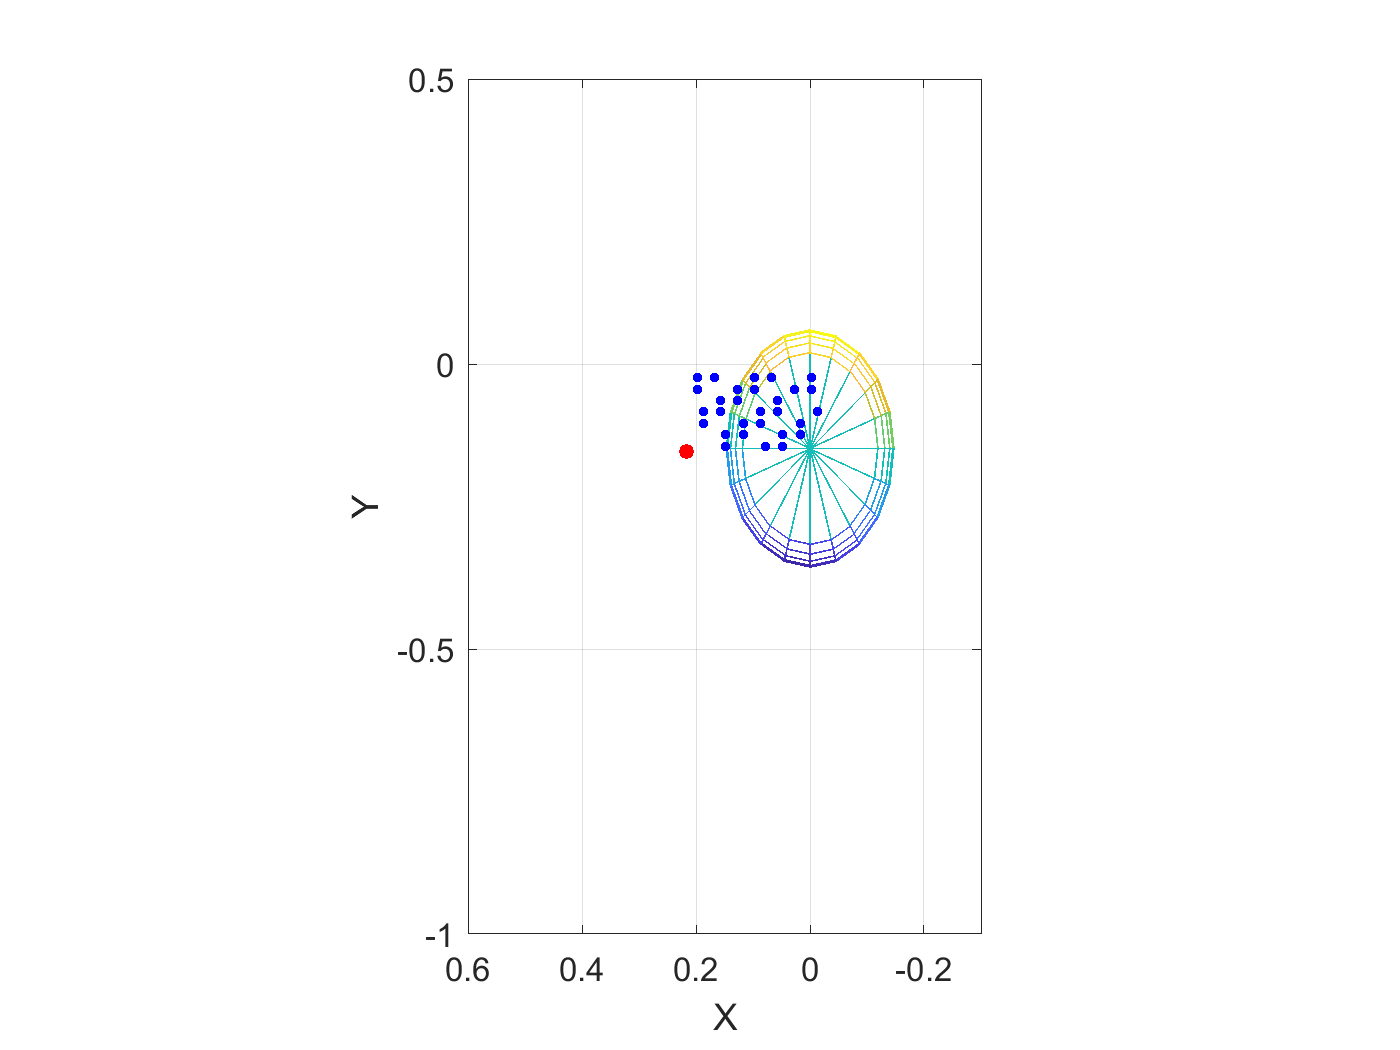
\includegraphics[width=0.6\textwidth]{Pictures/Results/Controller/DesiredPointsFV.png}
    \end{subfigure}
    \hfill
    %\vspace{1cm} % Adjust the space between the figures as needed
    \begin{subfigure}[b]{0.45\linewidth}            
        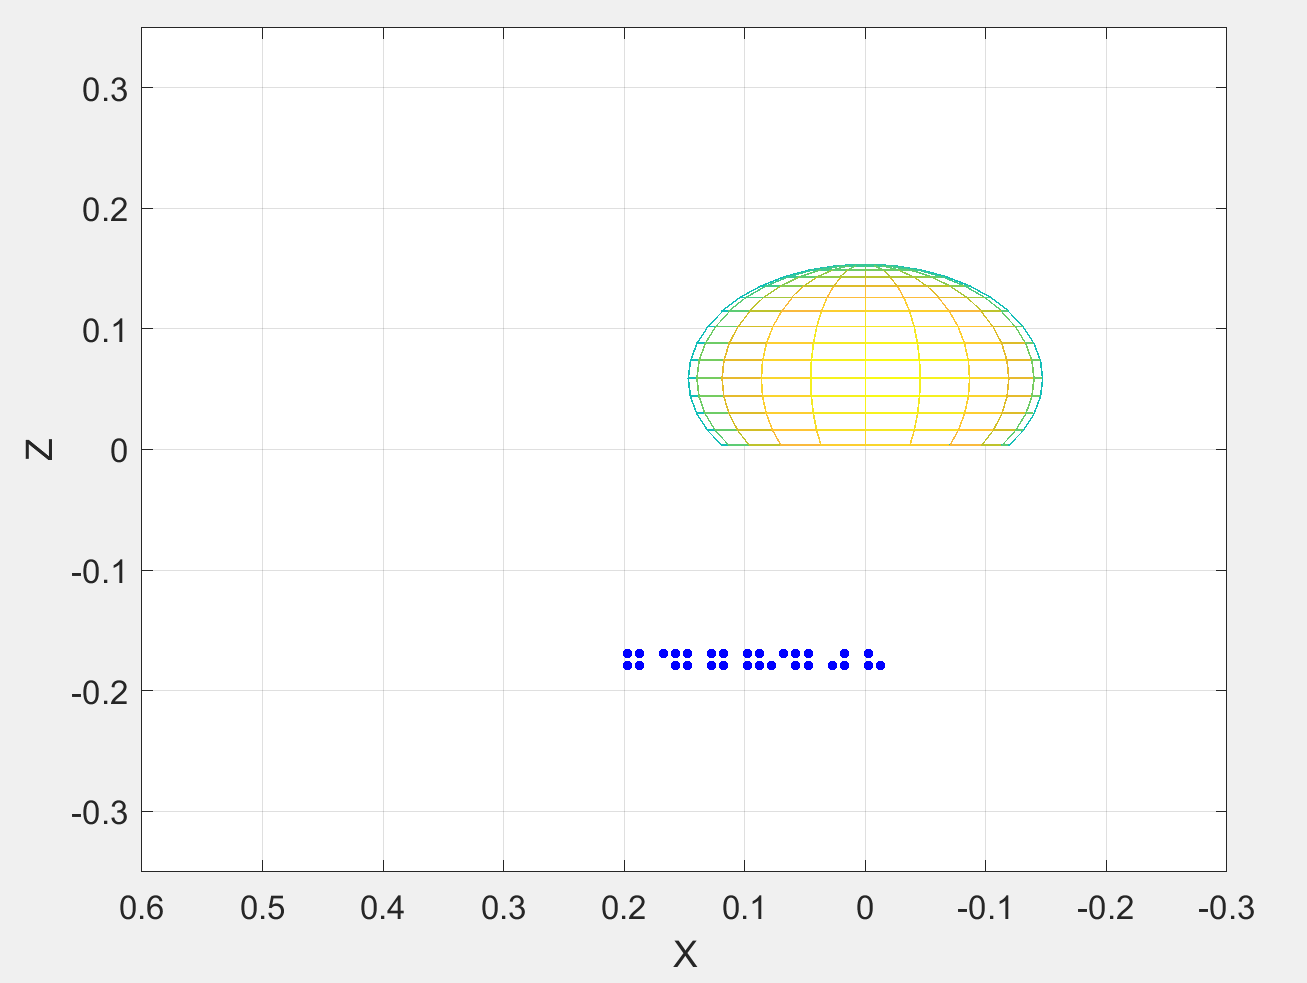
\includegraphics[width=0.7\textwidth]{Pictures/Results/Controller/DesiredPointsSV.png}
    \end{subfigure}
    \caption{Desired Targets for Reaching in Rehabilitation Task (Front View, Side View)}
    \label{fig:desiredpoints}
\end{figure}

Figure \ref{fig:allcontrollers} provides an initial overview of the different controllers operating at the same point. The progression begins with the static controller, transitions to path-following for the target point, and then introduces the stroke factor, affecting the arm's movement. In the final layer, the EMG-Influenced FES controller is integrated with the stroke-affected movement, allowing the arm to execute motions similar to those in a non-stroke scenario.

\begin{figure}[ht]
    \centering

    % Row 1, Column 1
    \begin{subfigure}[b]{0.5\textwidth}
        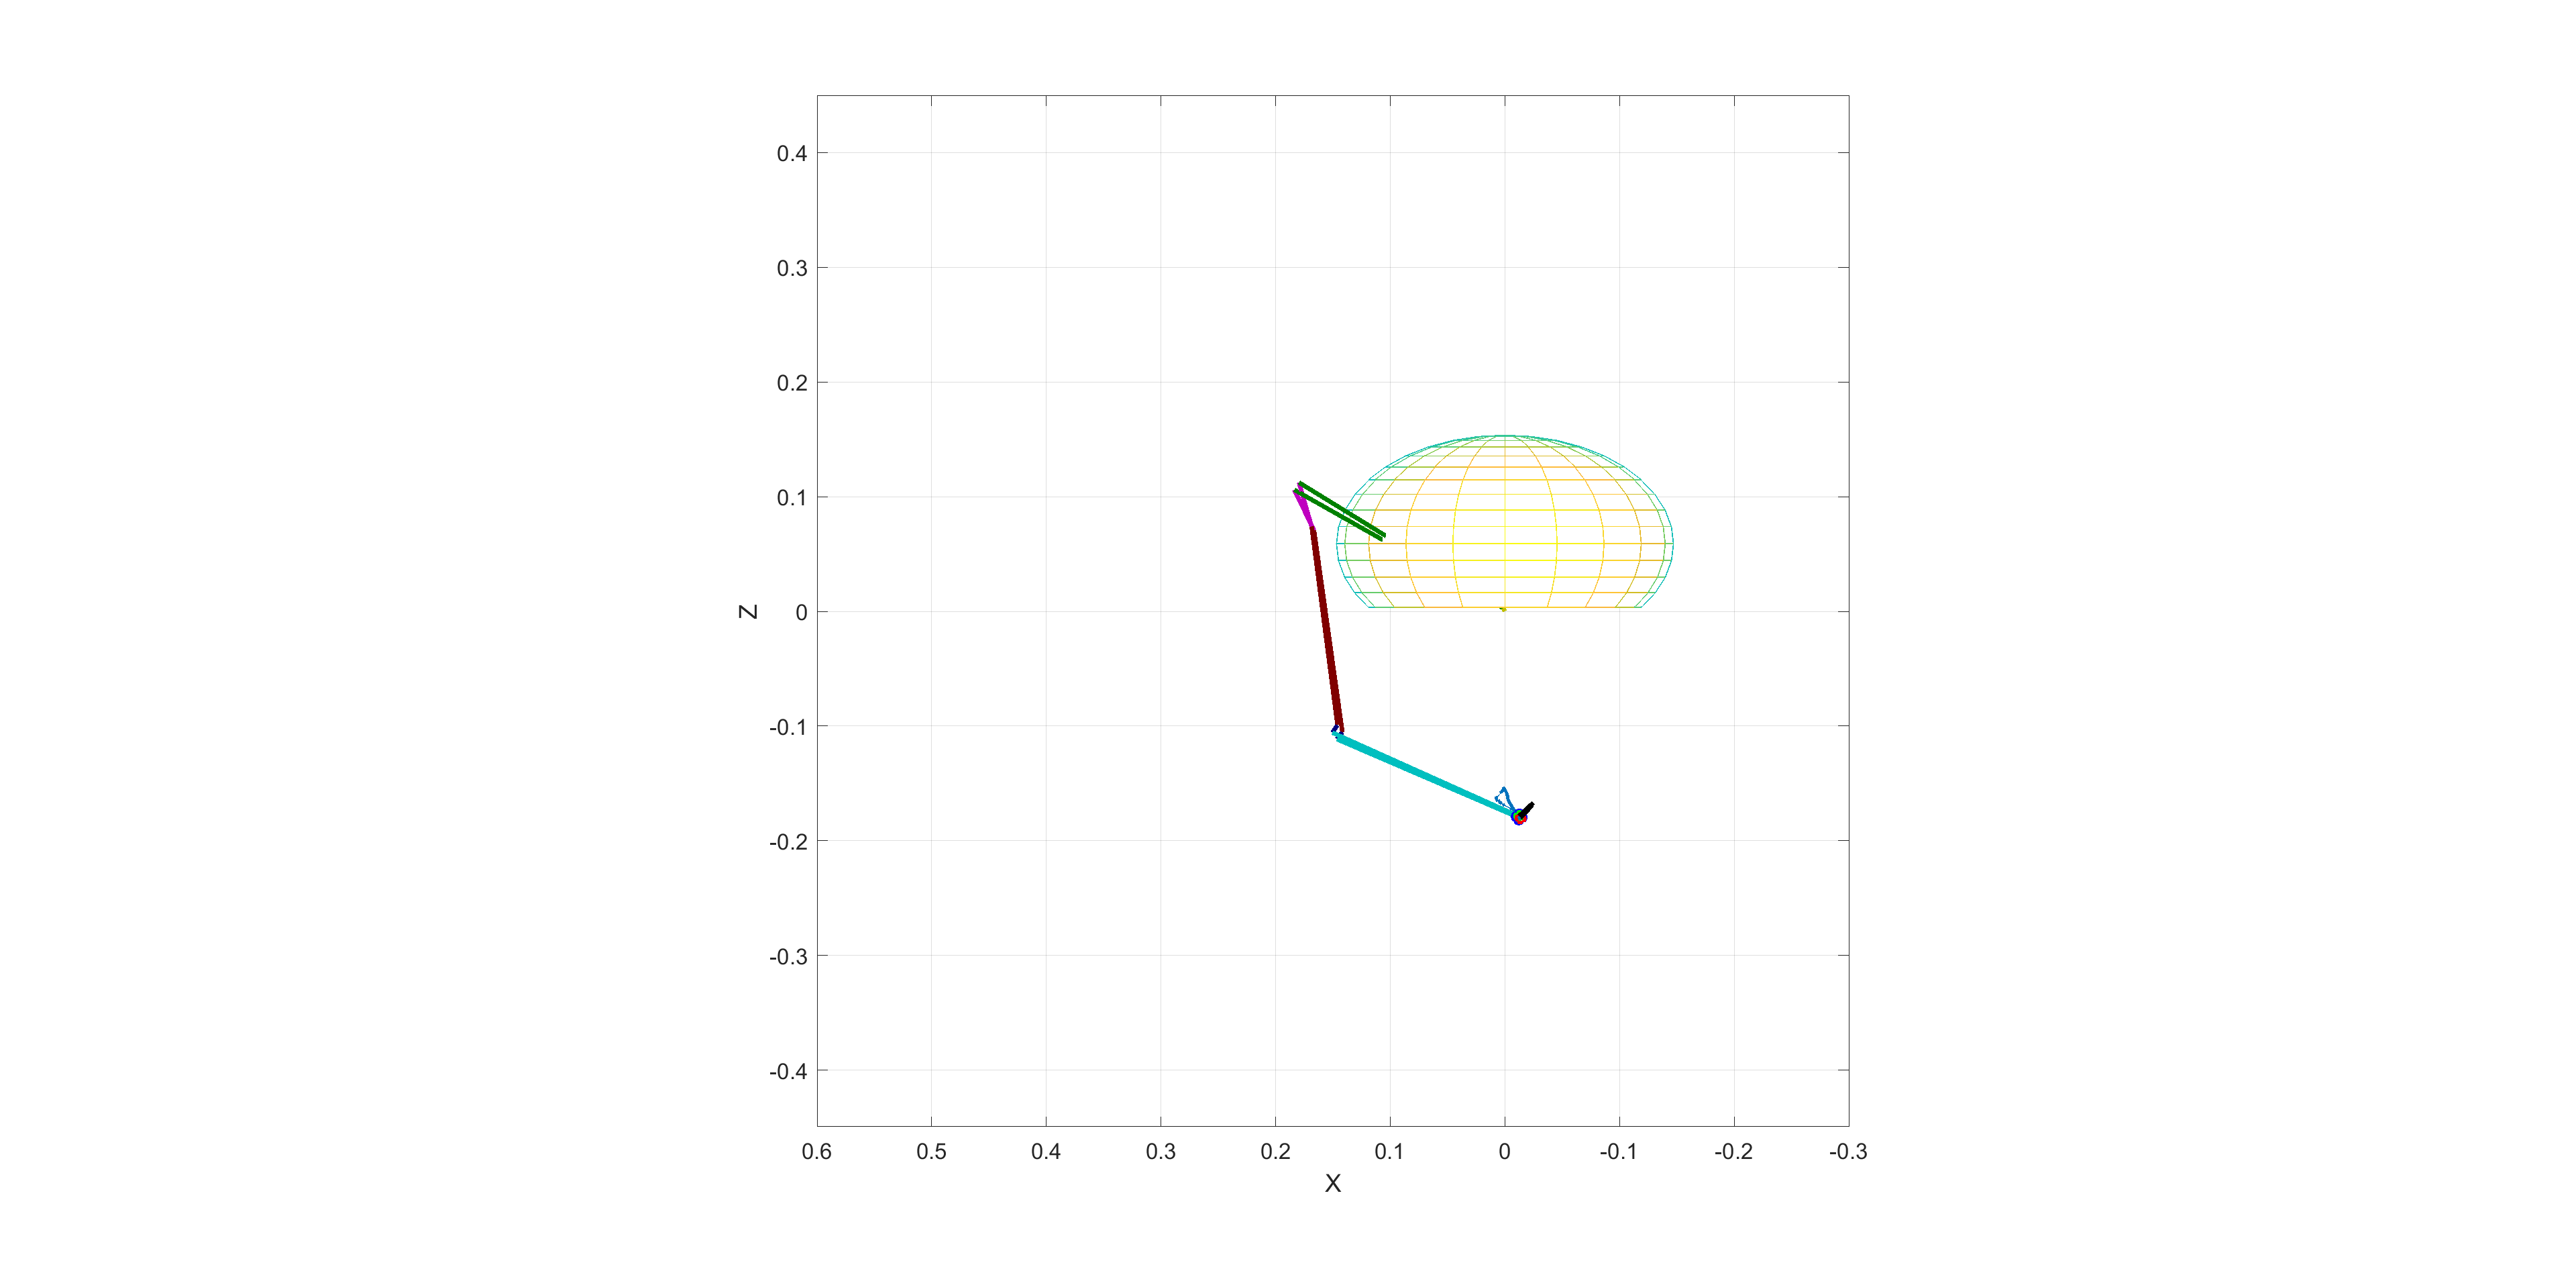
\includegraphics[width=0.75\linewidth]{Pictures/Controller/StaticControl_WP.png}
        \caption{Static Controller                                   }
    \end{subfigure}%
    \hfill
    % Row 1, Column 2
    \begin{subfigure}[b]{0.5\textwidth}
        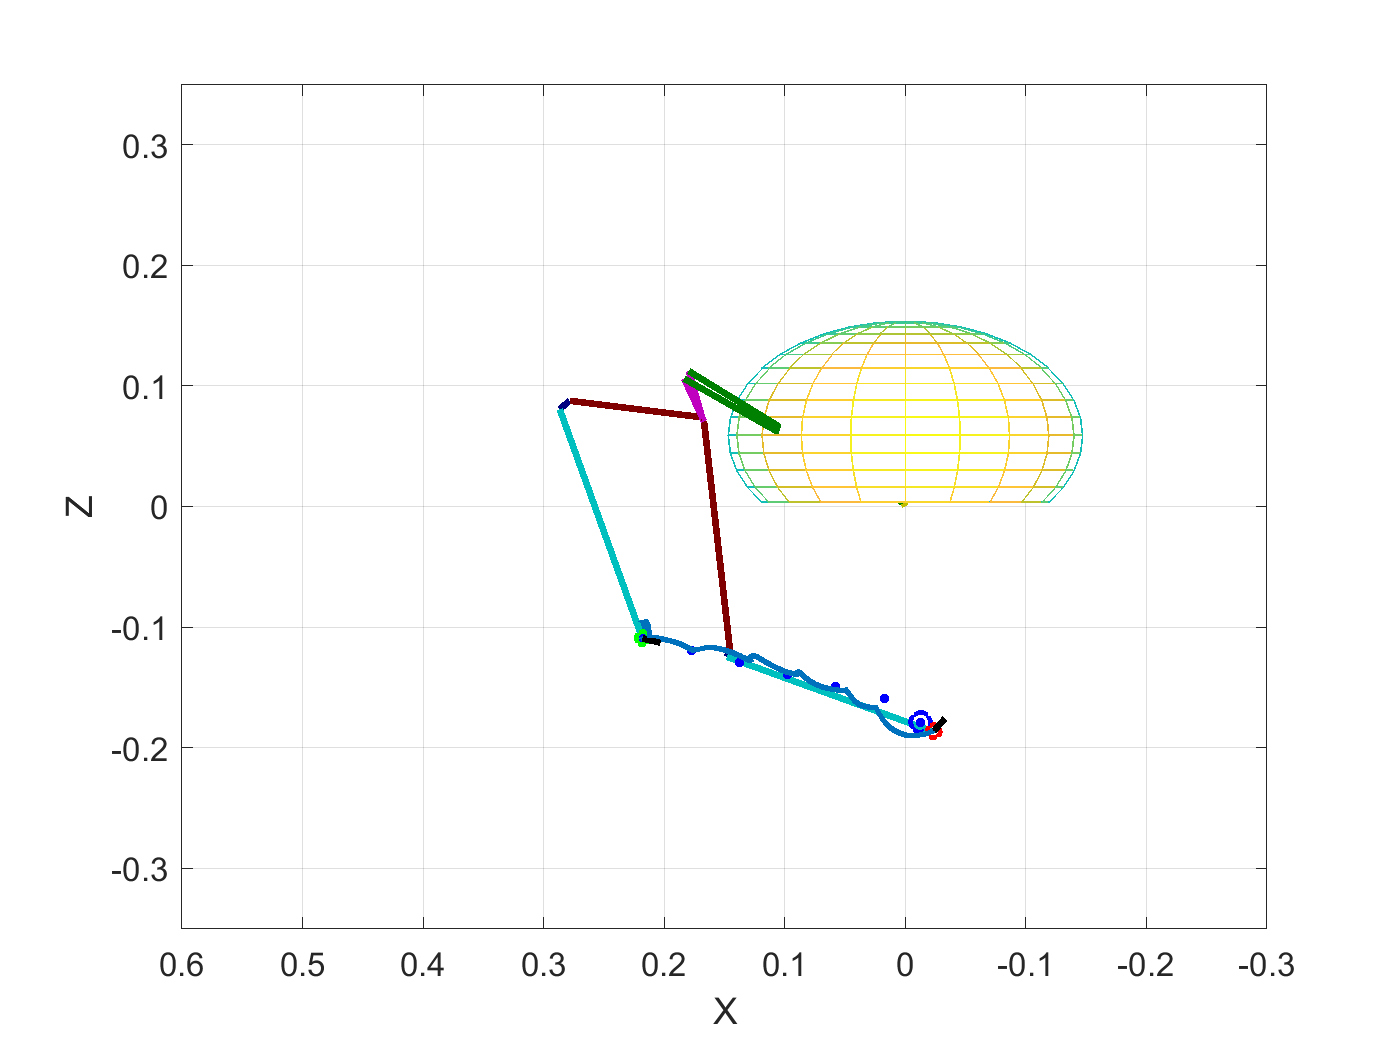
\includegraphics[width=0.75\linewidth]{Pictures/Controller/Healthy_WP.png}
        \caption{Non-Stroke Path-Following Quasi-Static Controller}
    \end{subfigure}

    \vspace{2pt} % Some vertical space between the rows

    % Row 2, Column 1
    \begin{subfigure}[b]{0.5\textwidth}
        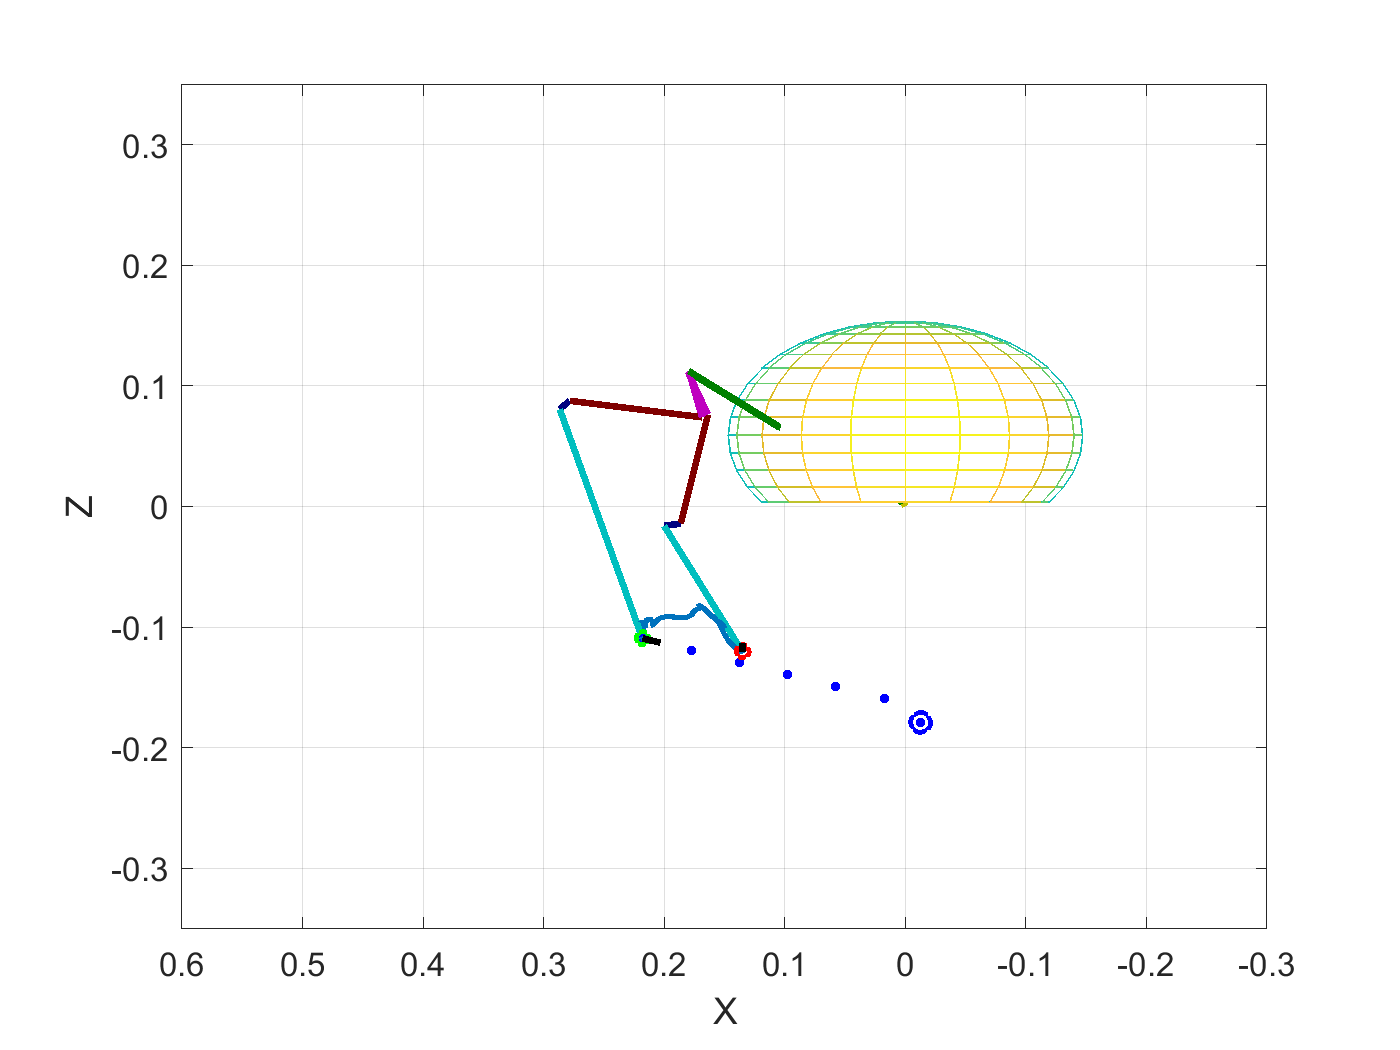
\includegraphics[width=0.75\linewidth]{Pictures/Results/Controller/StrokeWithouControl_WP.png}
        \caption{Stroke Path-Following Quasi-Static Controller}
    \end{subfigure}%
    \hfill
    % Row 2, Column 2
    \begin{subfigure}[b]{0.5\textwidth}
        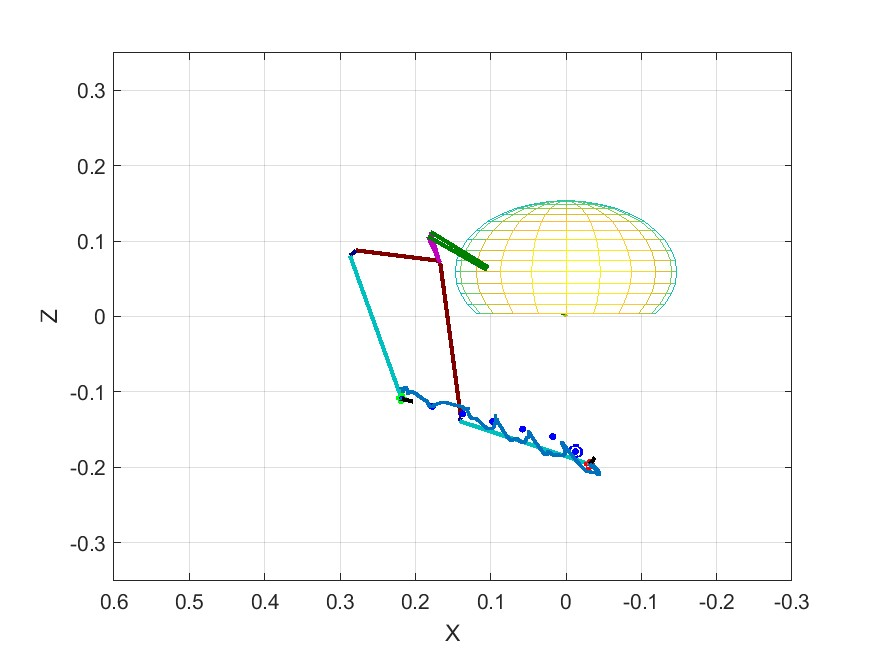
\includegraphics[width=0.75\linewidth]{Pictures/Results/Controller/G(2.99)_G(14.48)_Stroke_7_position_totry(5485)_wp.jpg}
        \caption{Stroke EMG-Influenced Quasi-Static Controller}
    \end{subfigure}

    \caption{Wrist Position Plots over Time}
    \label{fig:allcontrollers}
\end{figure}

\newpage
\subsection{Static Control} \label{resultsstaticcontrol}
The PI tuning was done with half of the desired points. However, the results shown in the table below show the error and variance of the target positions for all the desired targets. It can be seen that the higher Kp value reduces the variance and the mean target error. Moreover, it can be seen from the results and also from the plots on Figure \ref{fig:staticPItuning} that the steady state error is reduced by the introduction of integrating value. 

In Figure \ref{29statics}, we present the performance results of the Static Controller across all 29 positions. Furthermore, Figure \ref{fig:SC} illustrates the temporal variations in muscle forces and neural excitations for the triceps, deltoids, and biceps. This figure also emphasizes the efficacy of the PD controller, showcasing the feedback force which is subsequently converted to feedback torque, assisting in maintaining the arm's static position.

\begin{figure}[h!]
\centering
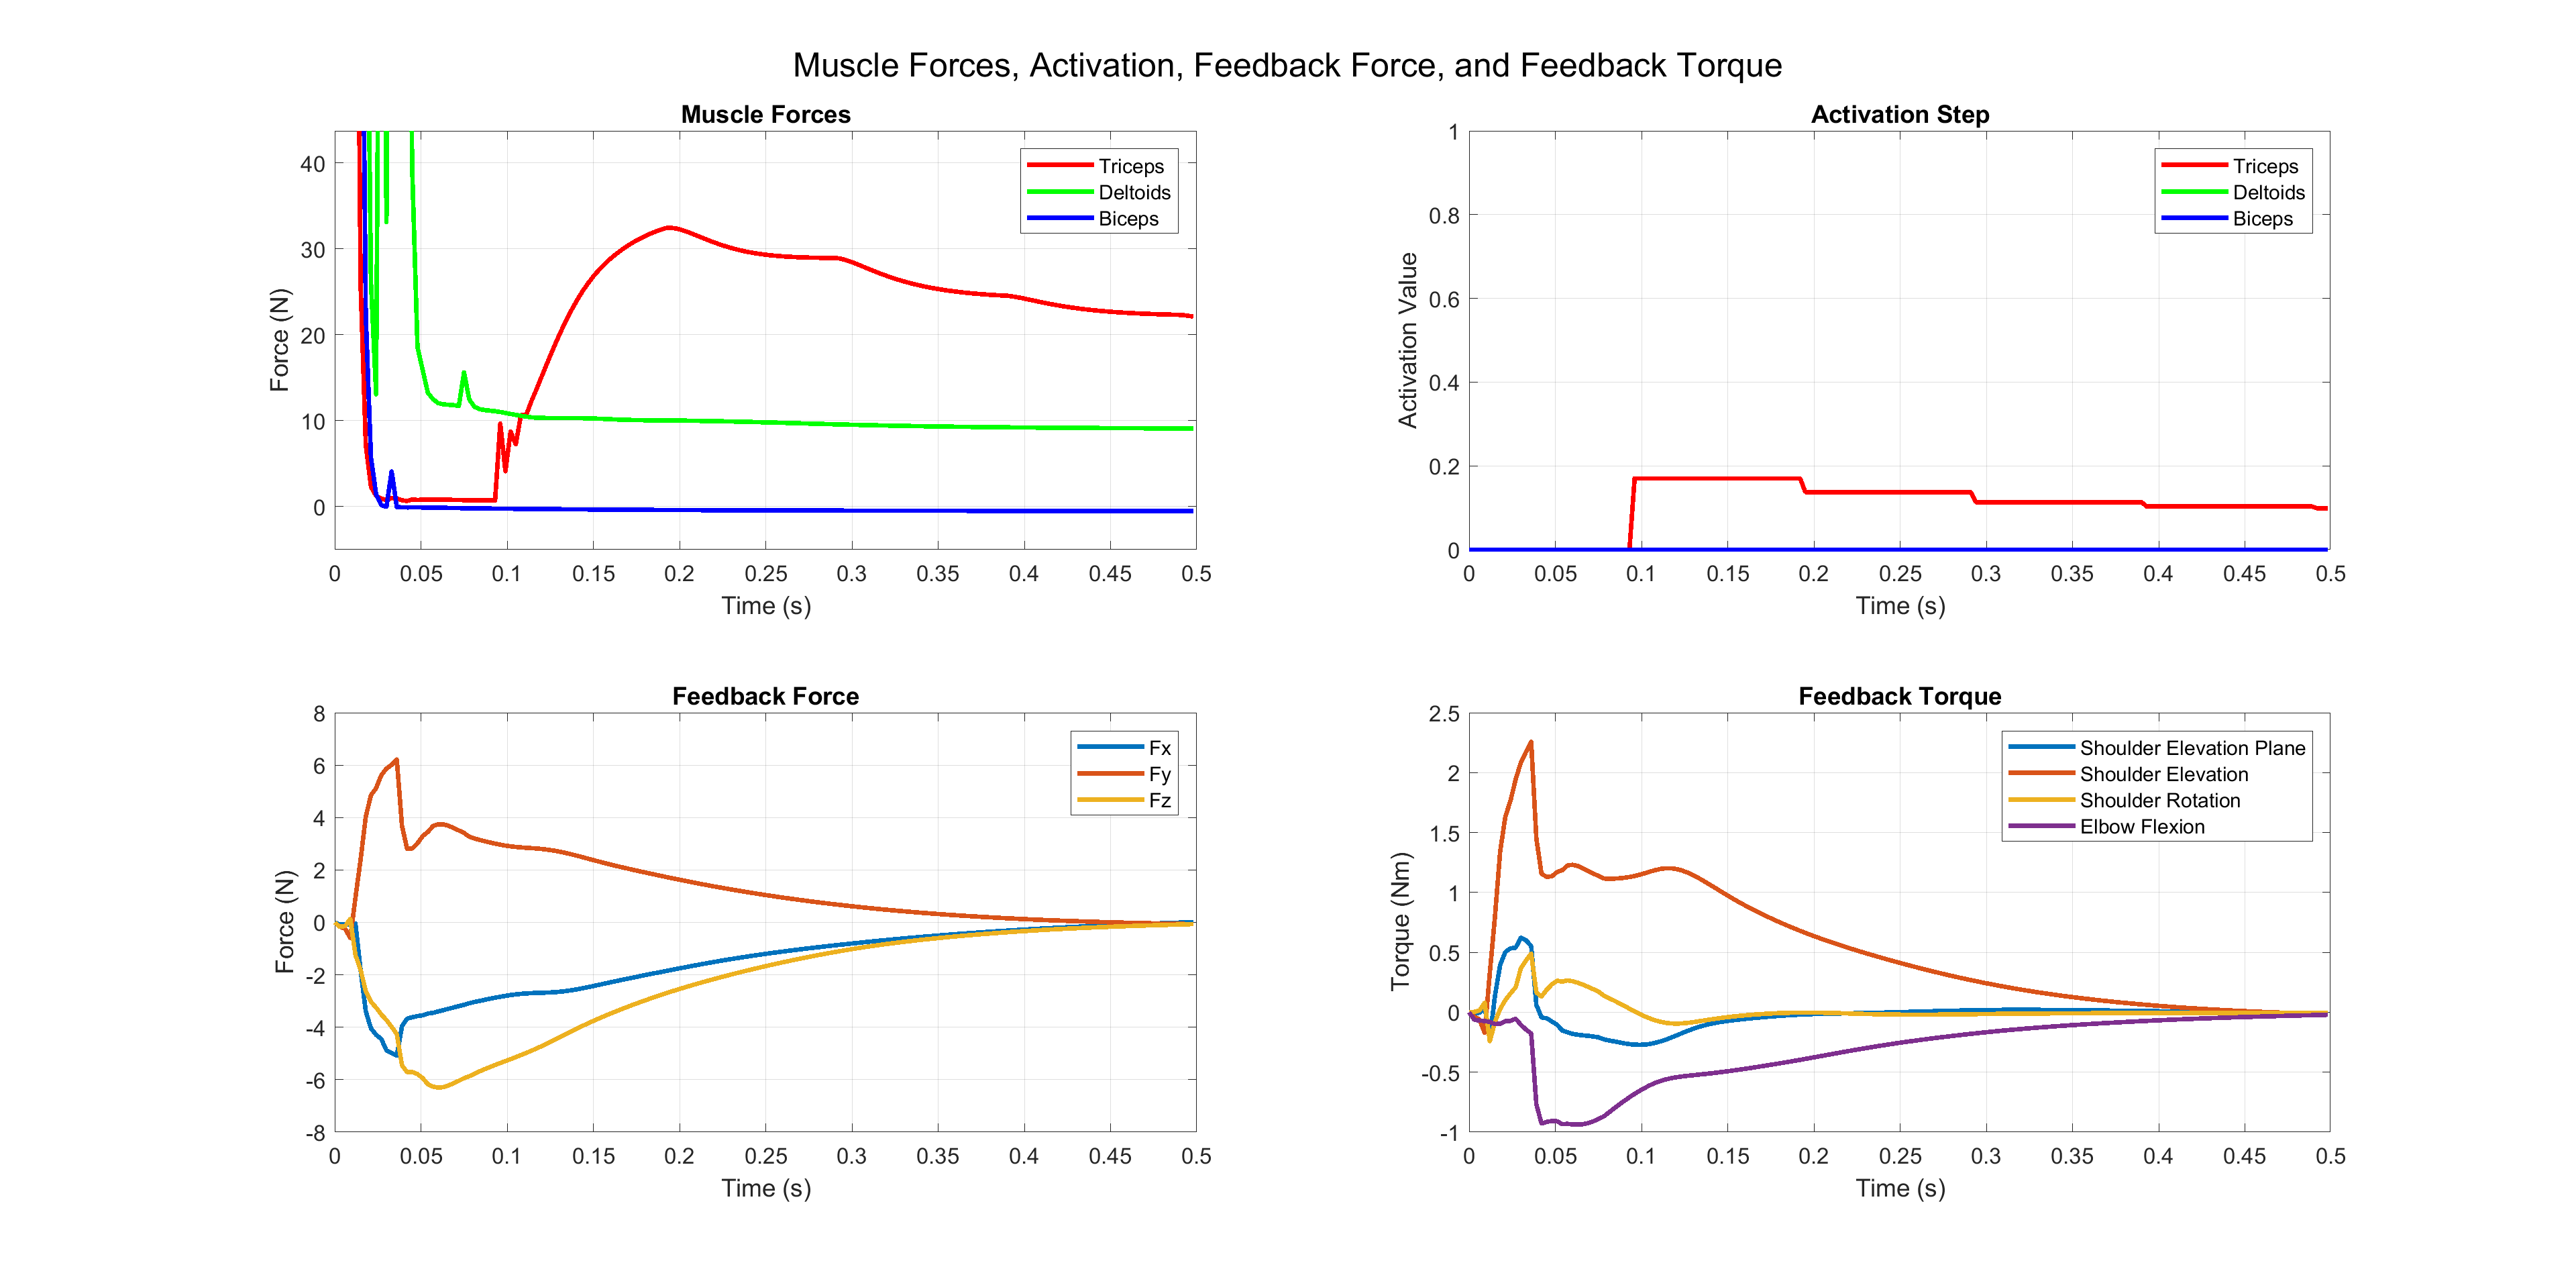
\includegraphics[width=1\textwidth]{Pictures/Controller/StaticControl.png} 
\caption{Static Control Example Muscle Forces, Activation Step, Feedback Force and Feedback Torque } % Optional caption
\label{fig:SC} % Optional label for referencing
\end{figure}

\begin{table}[h]
    \centering
    \tiny % Set font size
    \caption{Comparison between PI Values Results}
    \begin{tabularx}{\linewidth}{|X|X|X|}
        \hline
        \textbf{Controller} & \multicolumn{2}{c|}{\textbf{Target Position Error (m)}} \\
        \cline{2-3}
        & \textbf{Mean} & \textbf{Variance} \\
        \hline
        Kp = 100, Ki = 0 & [0.020 -0.026 0.003] & [0.060 0.238 0.025]$*10^{-3}$ \\
        \hline
        Kp = 100, Ki = 50  & [0.015 -0.021 0.003] & [0.046 0.160 0.024]$*10^{-3}$  \\
        \hline
        Kp = 300, Ki = 50 & [0.007 -0.012 0.002] & [0.012 0.041 0.013]$*10^{-3}$  \\
        \hline
        Kp = 300, Ki = 100 & [0.003 -0.012 -0.001] & [0.011 0.035 0.010]$*10^{-3}$  \\
        \hline
    \end{tabularx}
\end{table}

\begin{figure}[ht]
    \centering

    % Row 1, Column 1
    \begin{subfigure}[b]{0.45\textwidth}
        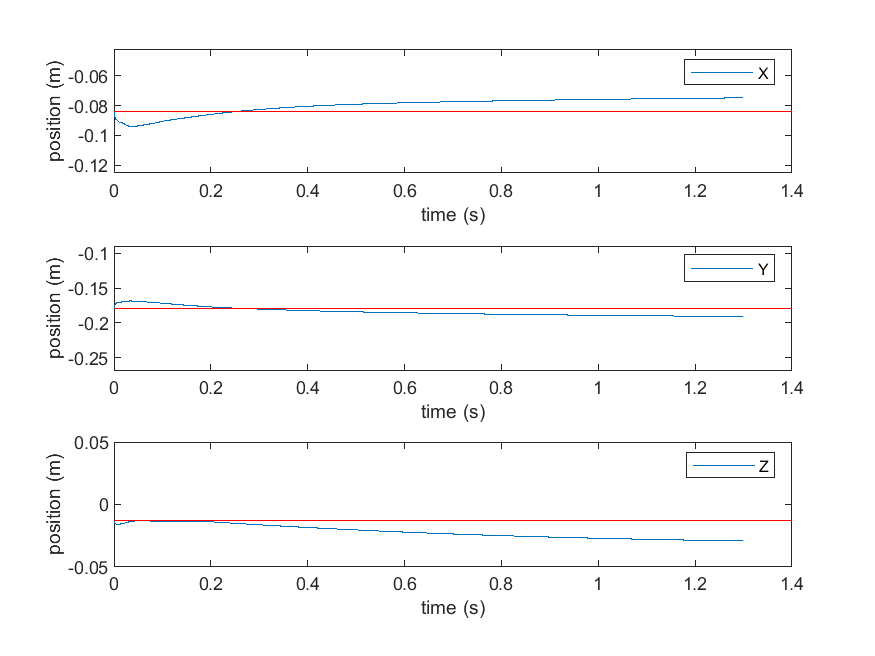
\includegraphics[width=\linewidth]{Pictures/Controller/Kp100Ki0/1.png}
        \caption{Position 1: Kp=100 Ki=0}
    \end{subfigure}%
    \hfill
    % Row 1, Column 2
    \begin{subfigure}[b]{0.45\textwidth}
        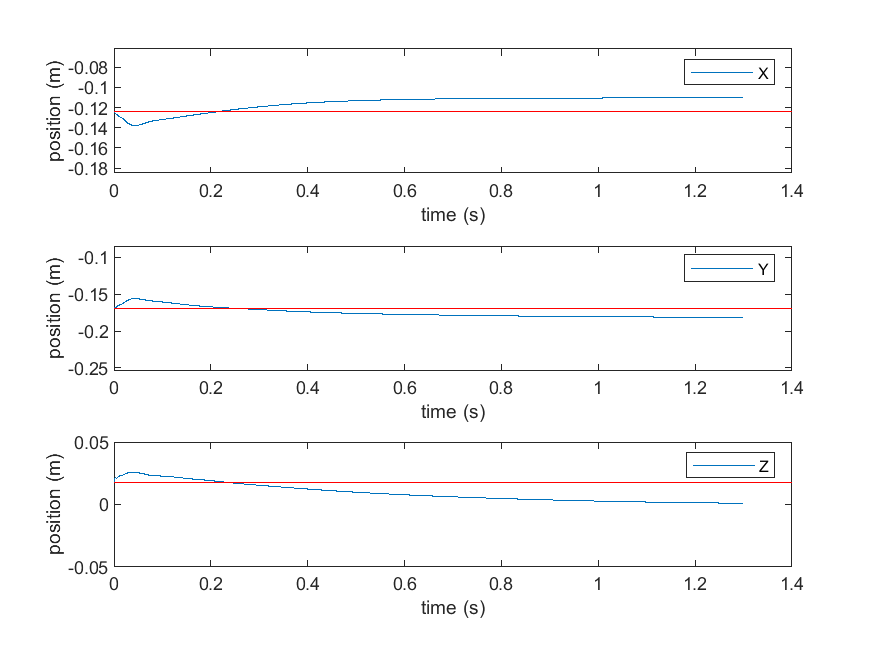
\includegraphics[width=\linewidth]{Pictures/Controller/Kp100Ki0/17.png}
        \caption{Position 2: Kp=100 Ki=0}
    \end{subfigure}

    \vspace{2pt} % Some vertical space between the rows

    % Row 2, Column 1
    \begin{subfigure}[b]{0.45\textwidth}
        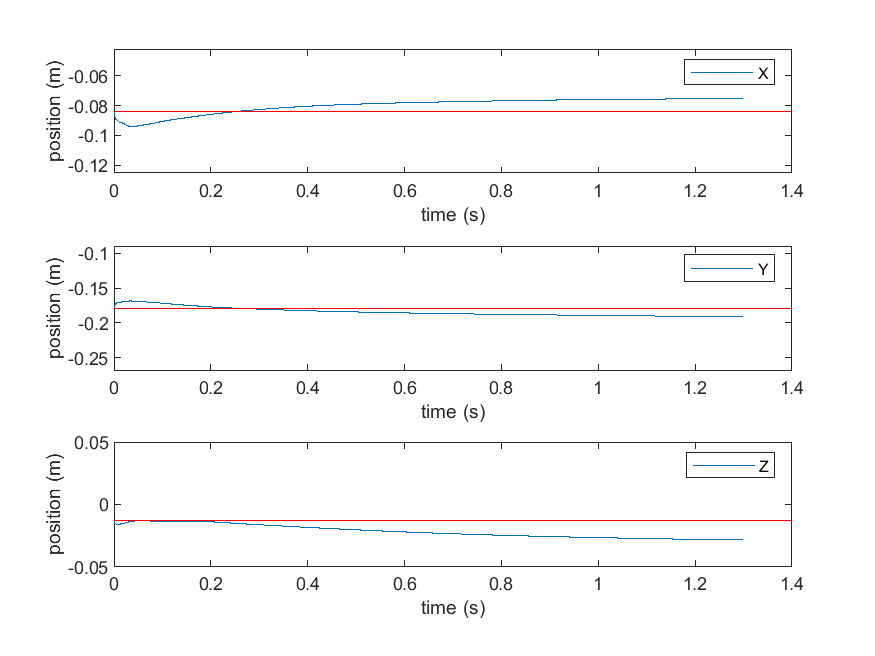
\includegraphics[width=\linewidth]{Pictures/Controller/Kp100Ki50/1.png}
        \caption{Position 1: Kp=100 Ki=50}
    \end{subfigure}%
    \hfill
    % Row 2, Column 2
    \begin{subfigure}[b]{0.45\textwidth}
        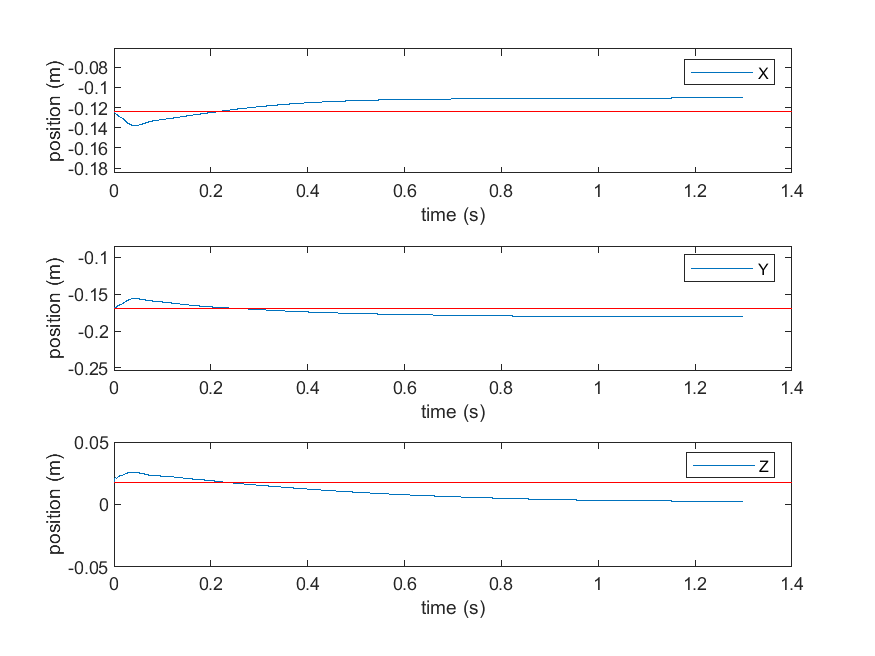
\includegraphics[width=\linewidth]{Pictures/Controller/Kp100Ki50/17.png}
        \caption{Position 2: Kp=100 Ki=50}
    \end{subfigure}

    \vspace{2pt} % Some vertical space between the rows

    % Row 3, Column 1
    \begin{subfigure}[b]{0.45\textwidth}
        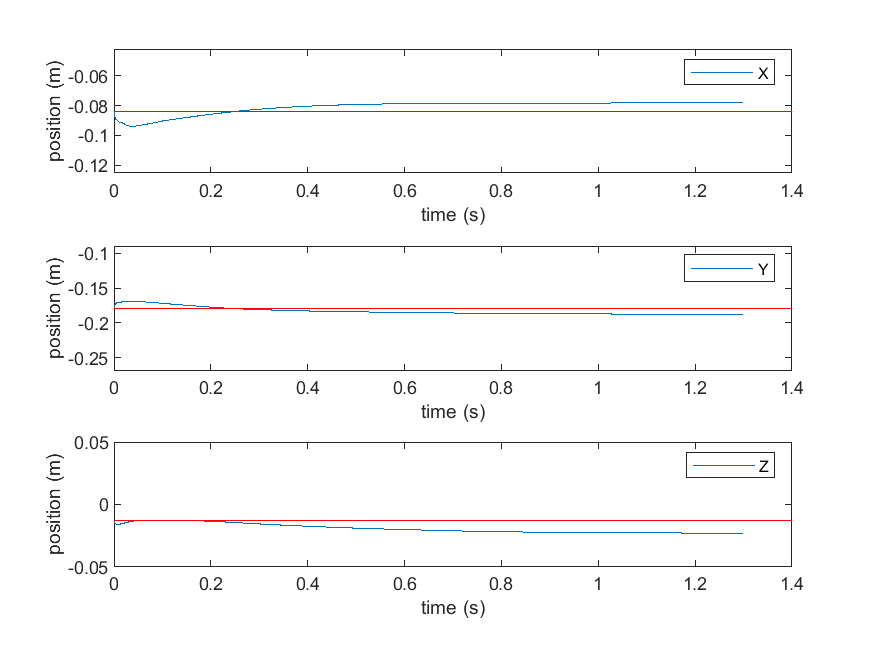
\includegraphics[width=\linewidth]{Pictures/Controller/Kp300Ki50/1.png}
        \caption{Position 1: Kp=300 Ki=50}
    \end{subfigure}%
    \hfill
    % Row 3, Column 2
    \begin{subfigure}[b]{0.45\textwidth}
        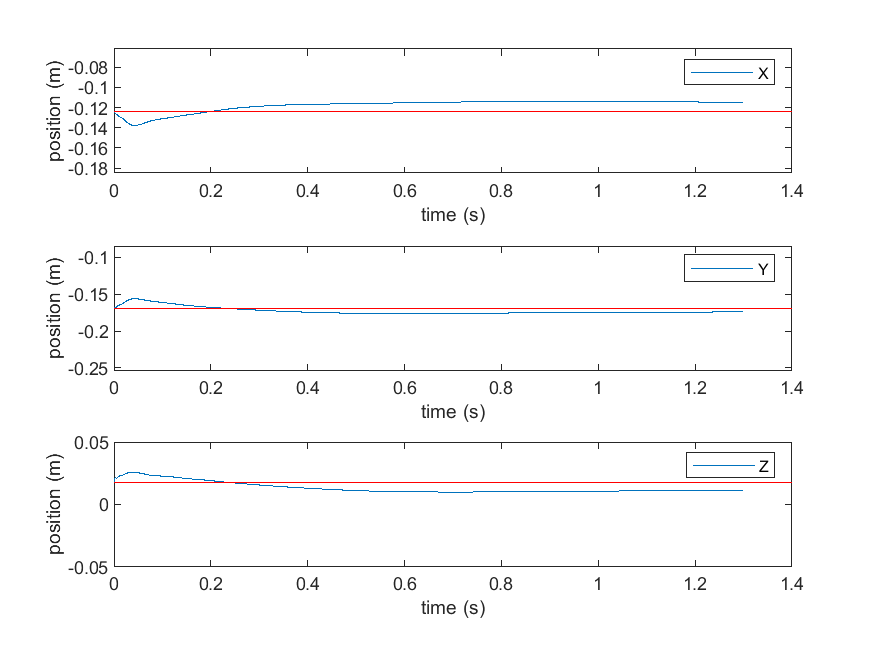
\includegraphics[width=\linewidth]{Pictures/Controller/Kp300Ki50/17.png}
        \caption{Position 2: Kp=300 Ki=50}
    \end{subfigure}

    \vspace{2pt} % Some vertical space between the rows

    % Row 4, Column 1
    \begin{subfigure}[b]{0.45\textwidth}
        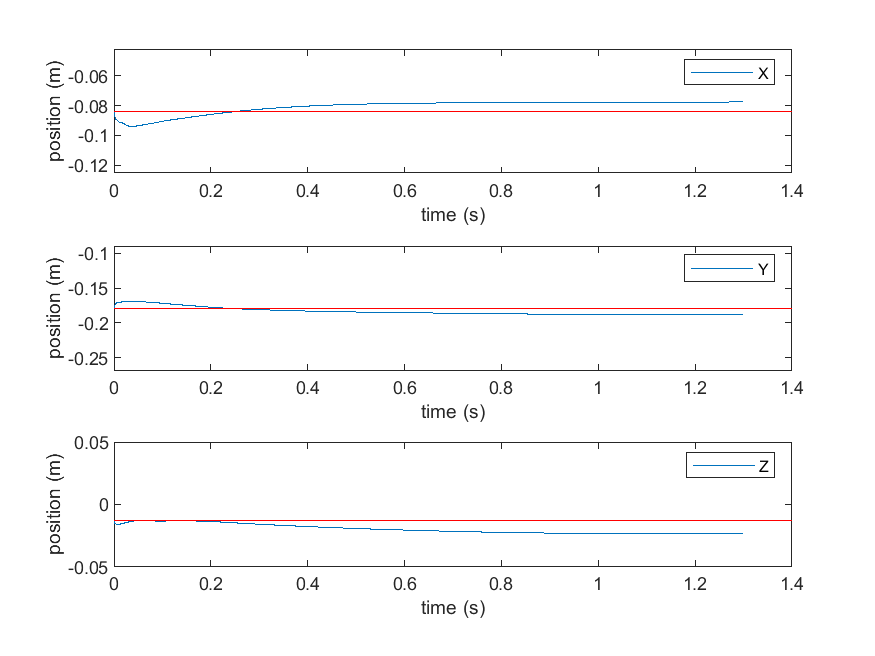
\includegraphics[width=\linewidth]{Pictures/Controller/Kp300Ki100/1.png}
        \caption{Position 1: Kp=300 Ki=100}
    \end{subfigure}%
    \hfill
    % Row 4, Column 2
    \begin{subfigure}[b]{0.45\textwidth}
        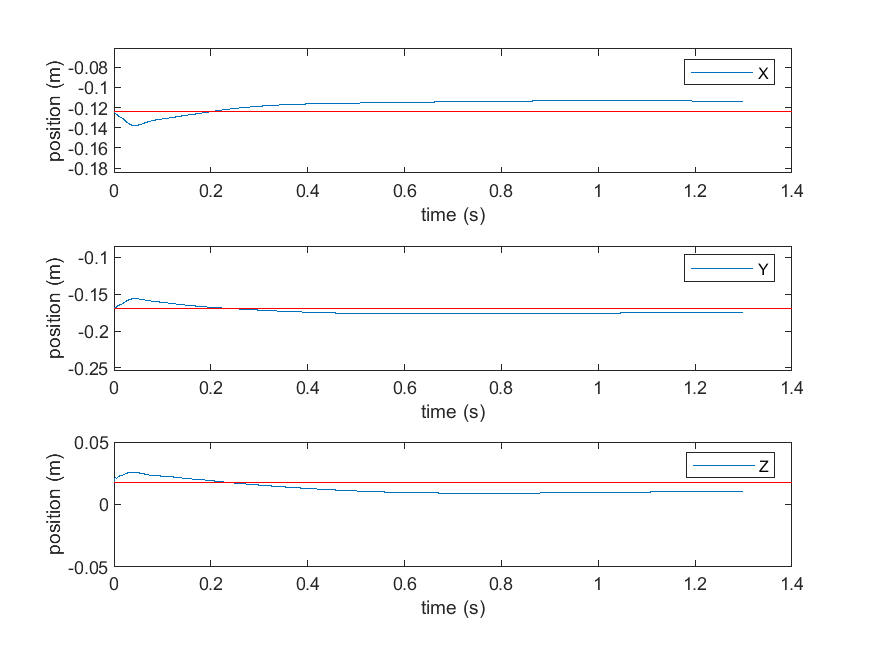
\includegraphics[width=\linewidth]{Pictures/Controller/Kp300Ki100/17.png}
        \caption{Position 2: Kp=300 Ki=100}
    \end{subfigure}

    \caption{Static Controller Different PI values for Tuning}
    \label{fig:staticPItuning}
\end{figure}


\newpage
\begin{landscape} % Start landscape page
  \begin{figure}[h!]
    \centering
    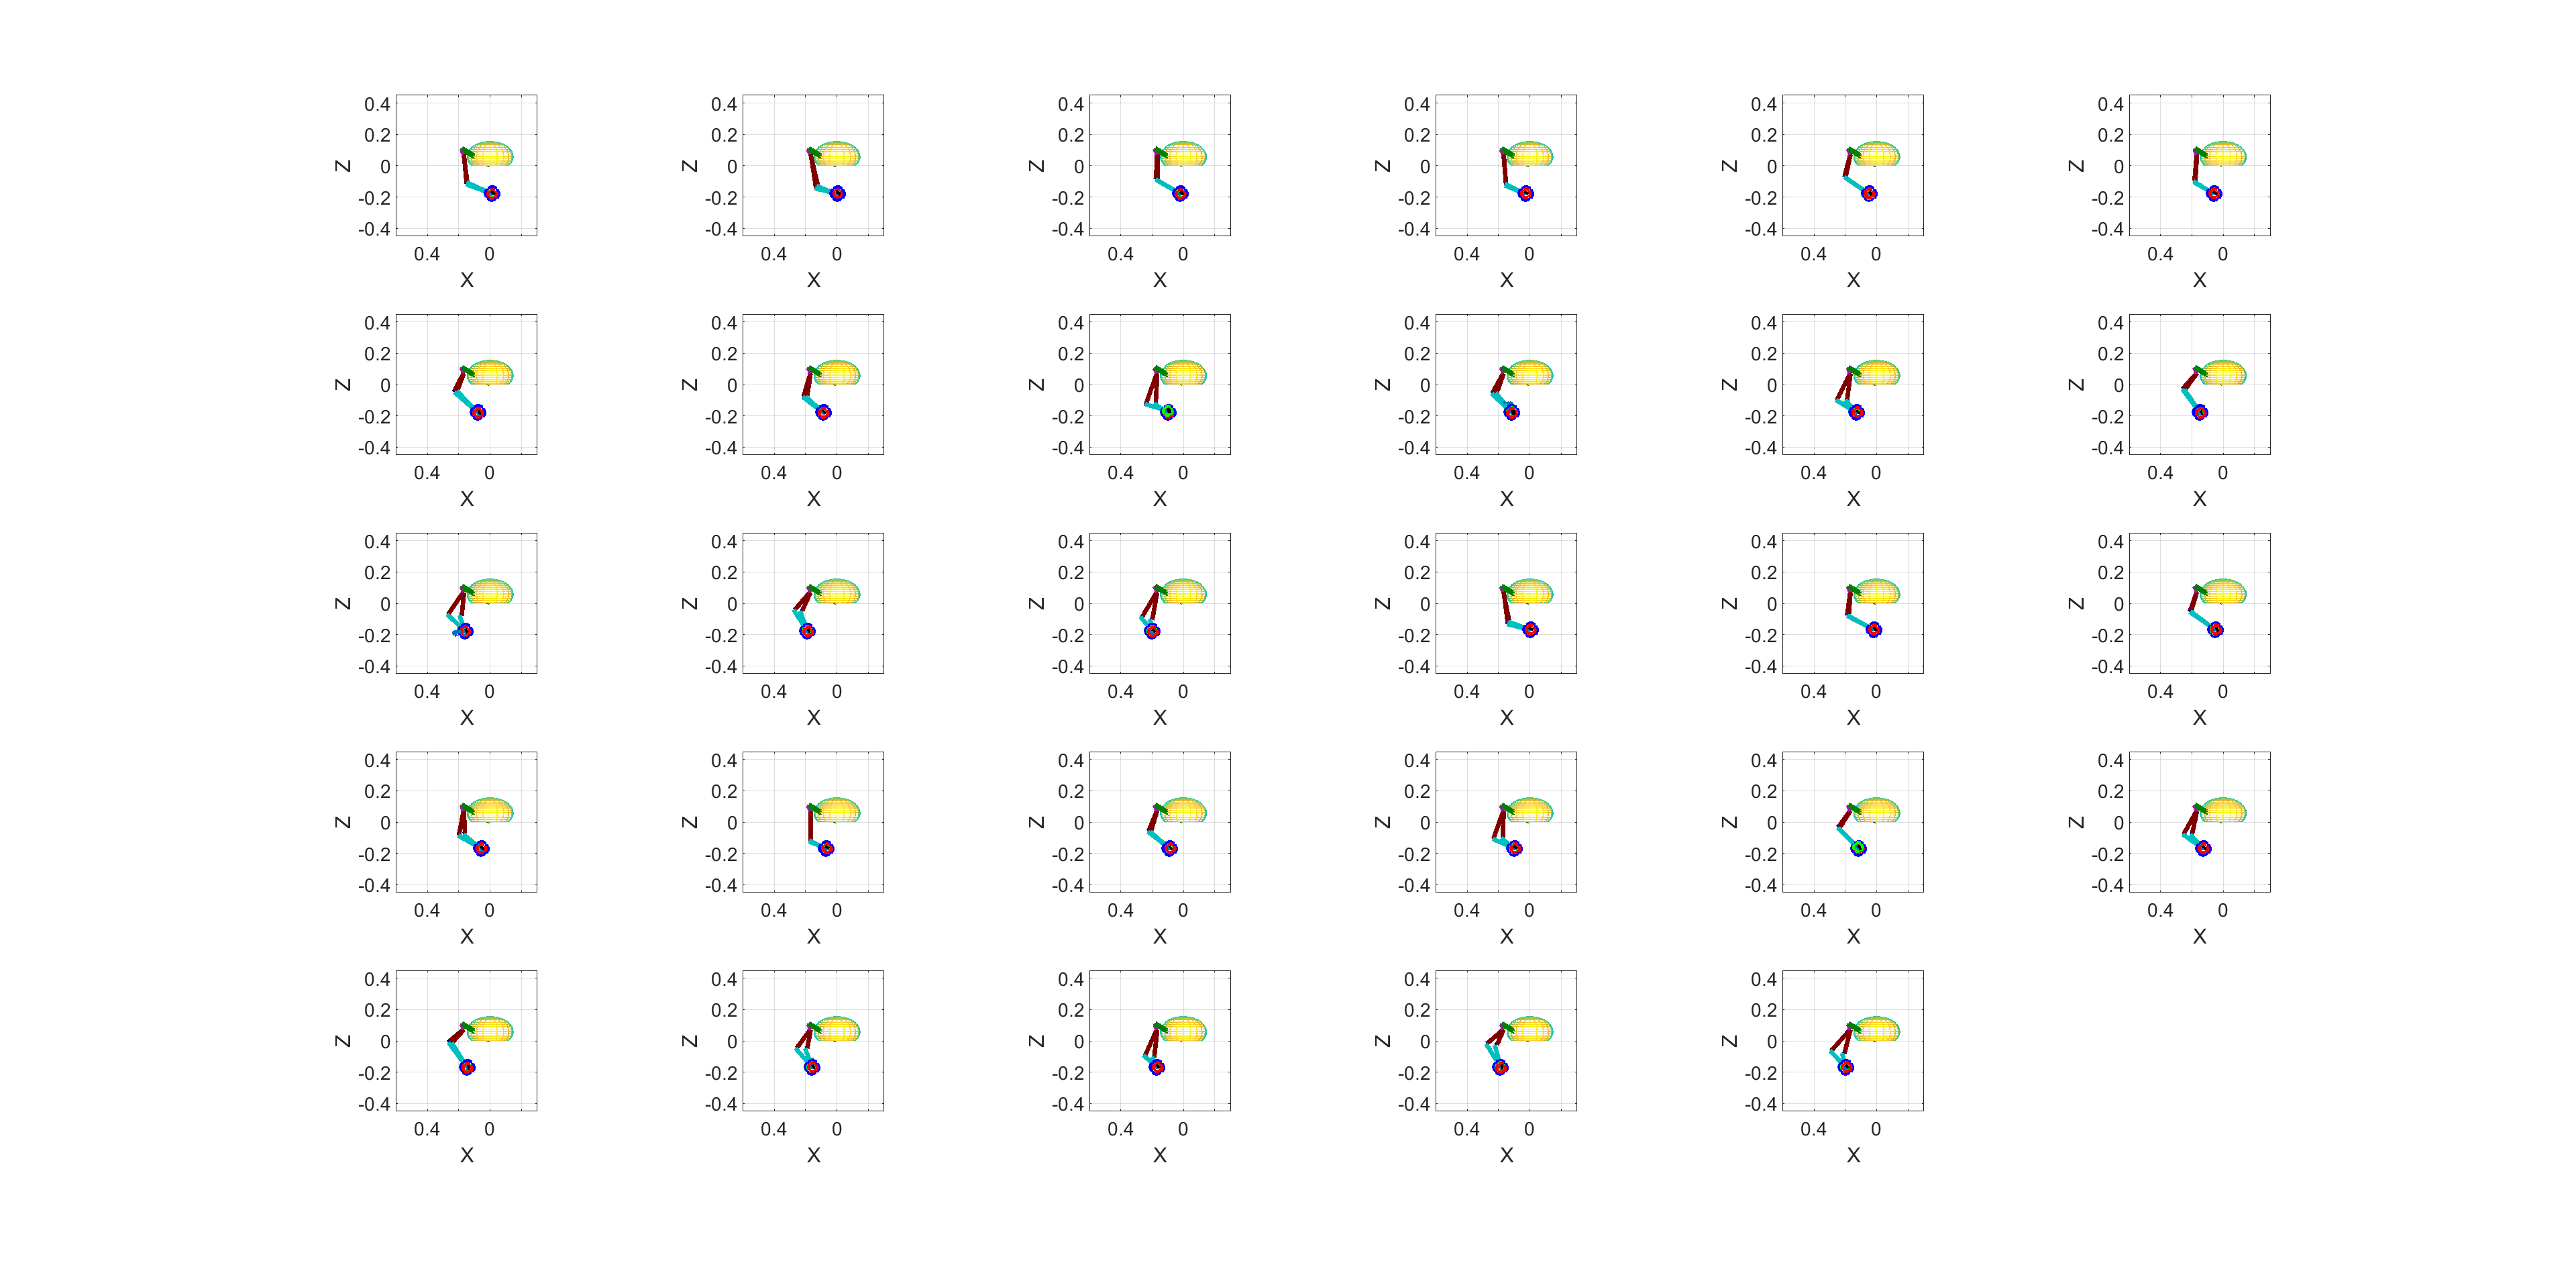
\includegraphics[width=1.9\textwidth]{Pictures/Controller/Static29positions.png} % Replace "filename.jpg" with the name of your image file
    \caption{Desired Targets in Static Control} % Optional caption
    \label{29statics}

  \end{figure}
\end{landscape} % End landscape page




\subsection{Path Following Quasi-Static Control}
\begin{figure}[h!]
\centering
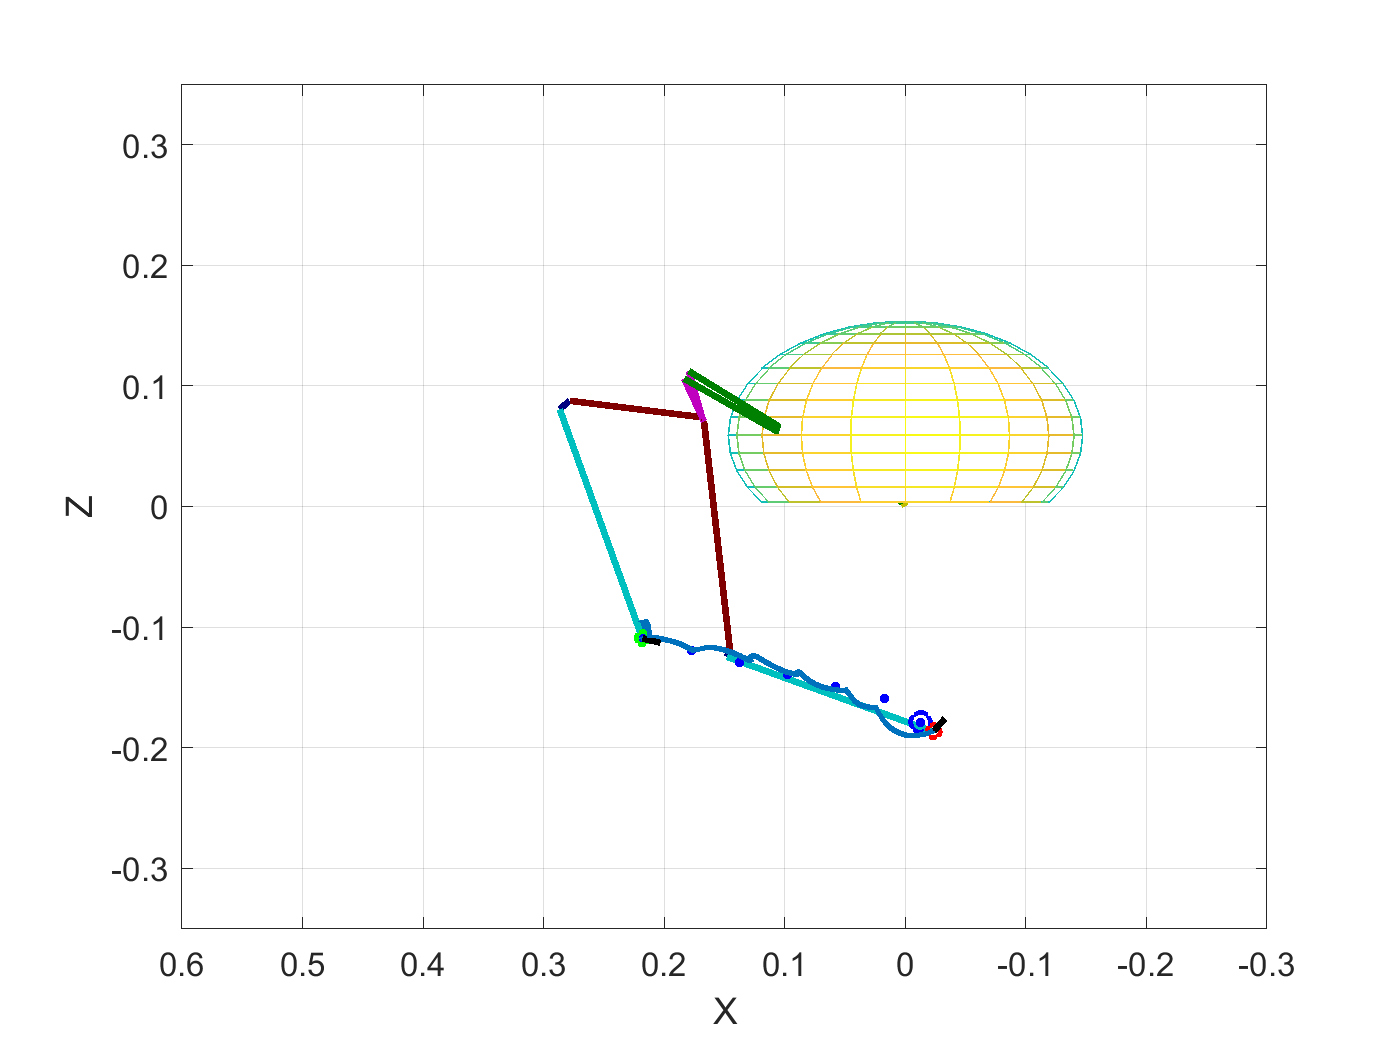
\includegraphics[width=0.75\textwidth]{Pictures/Controller/Healthy_WP.png} 
\caption{Path Following Quasi-Static Control Wrist Position} % Optional caption
\label{fig:PFWP} % Optional label for referencing
\end{figure}

\begin{figure}[h!]
\centering
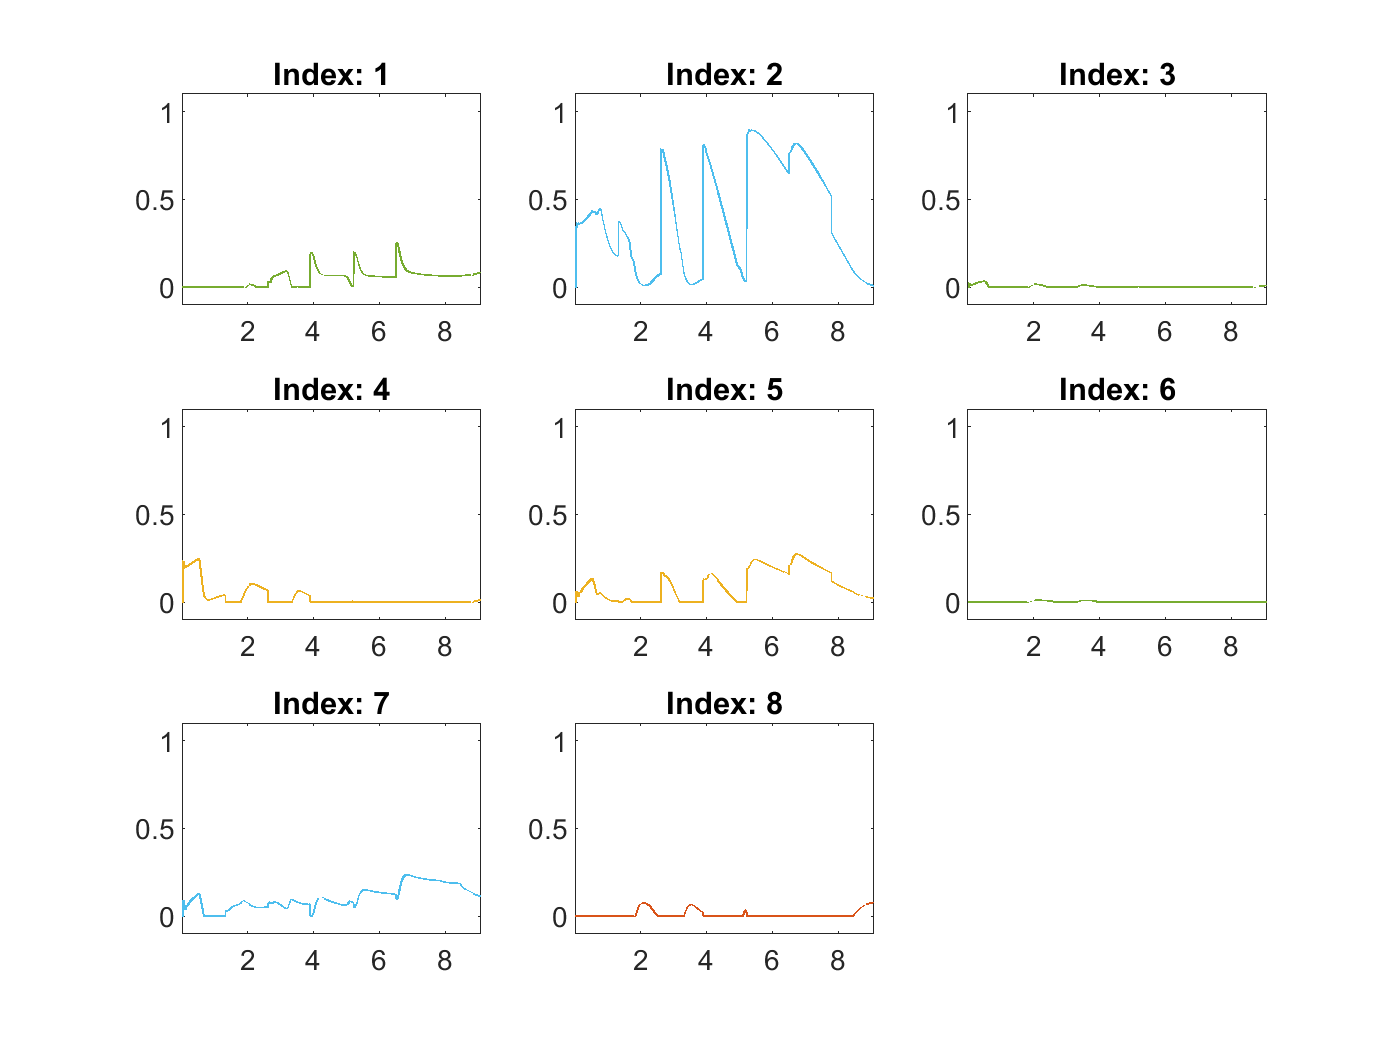
\includegraphics[width=1\textwidth]{Pictures/Controller/Healthy_NA.png} 
\caption{Path Following Quasi-Static Control Neural Activation} % Optional caption
\label{fig:PFNA} % Optional label for referencing
\end{figure}

\newpage
\begin{landscape} % Start landscape page
  \begin{figure}[h!]
    \centering
    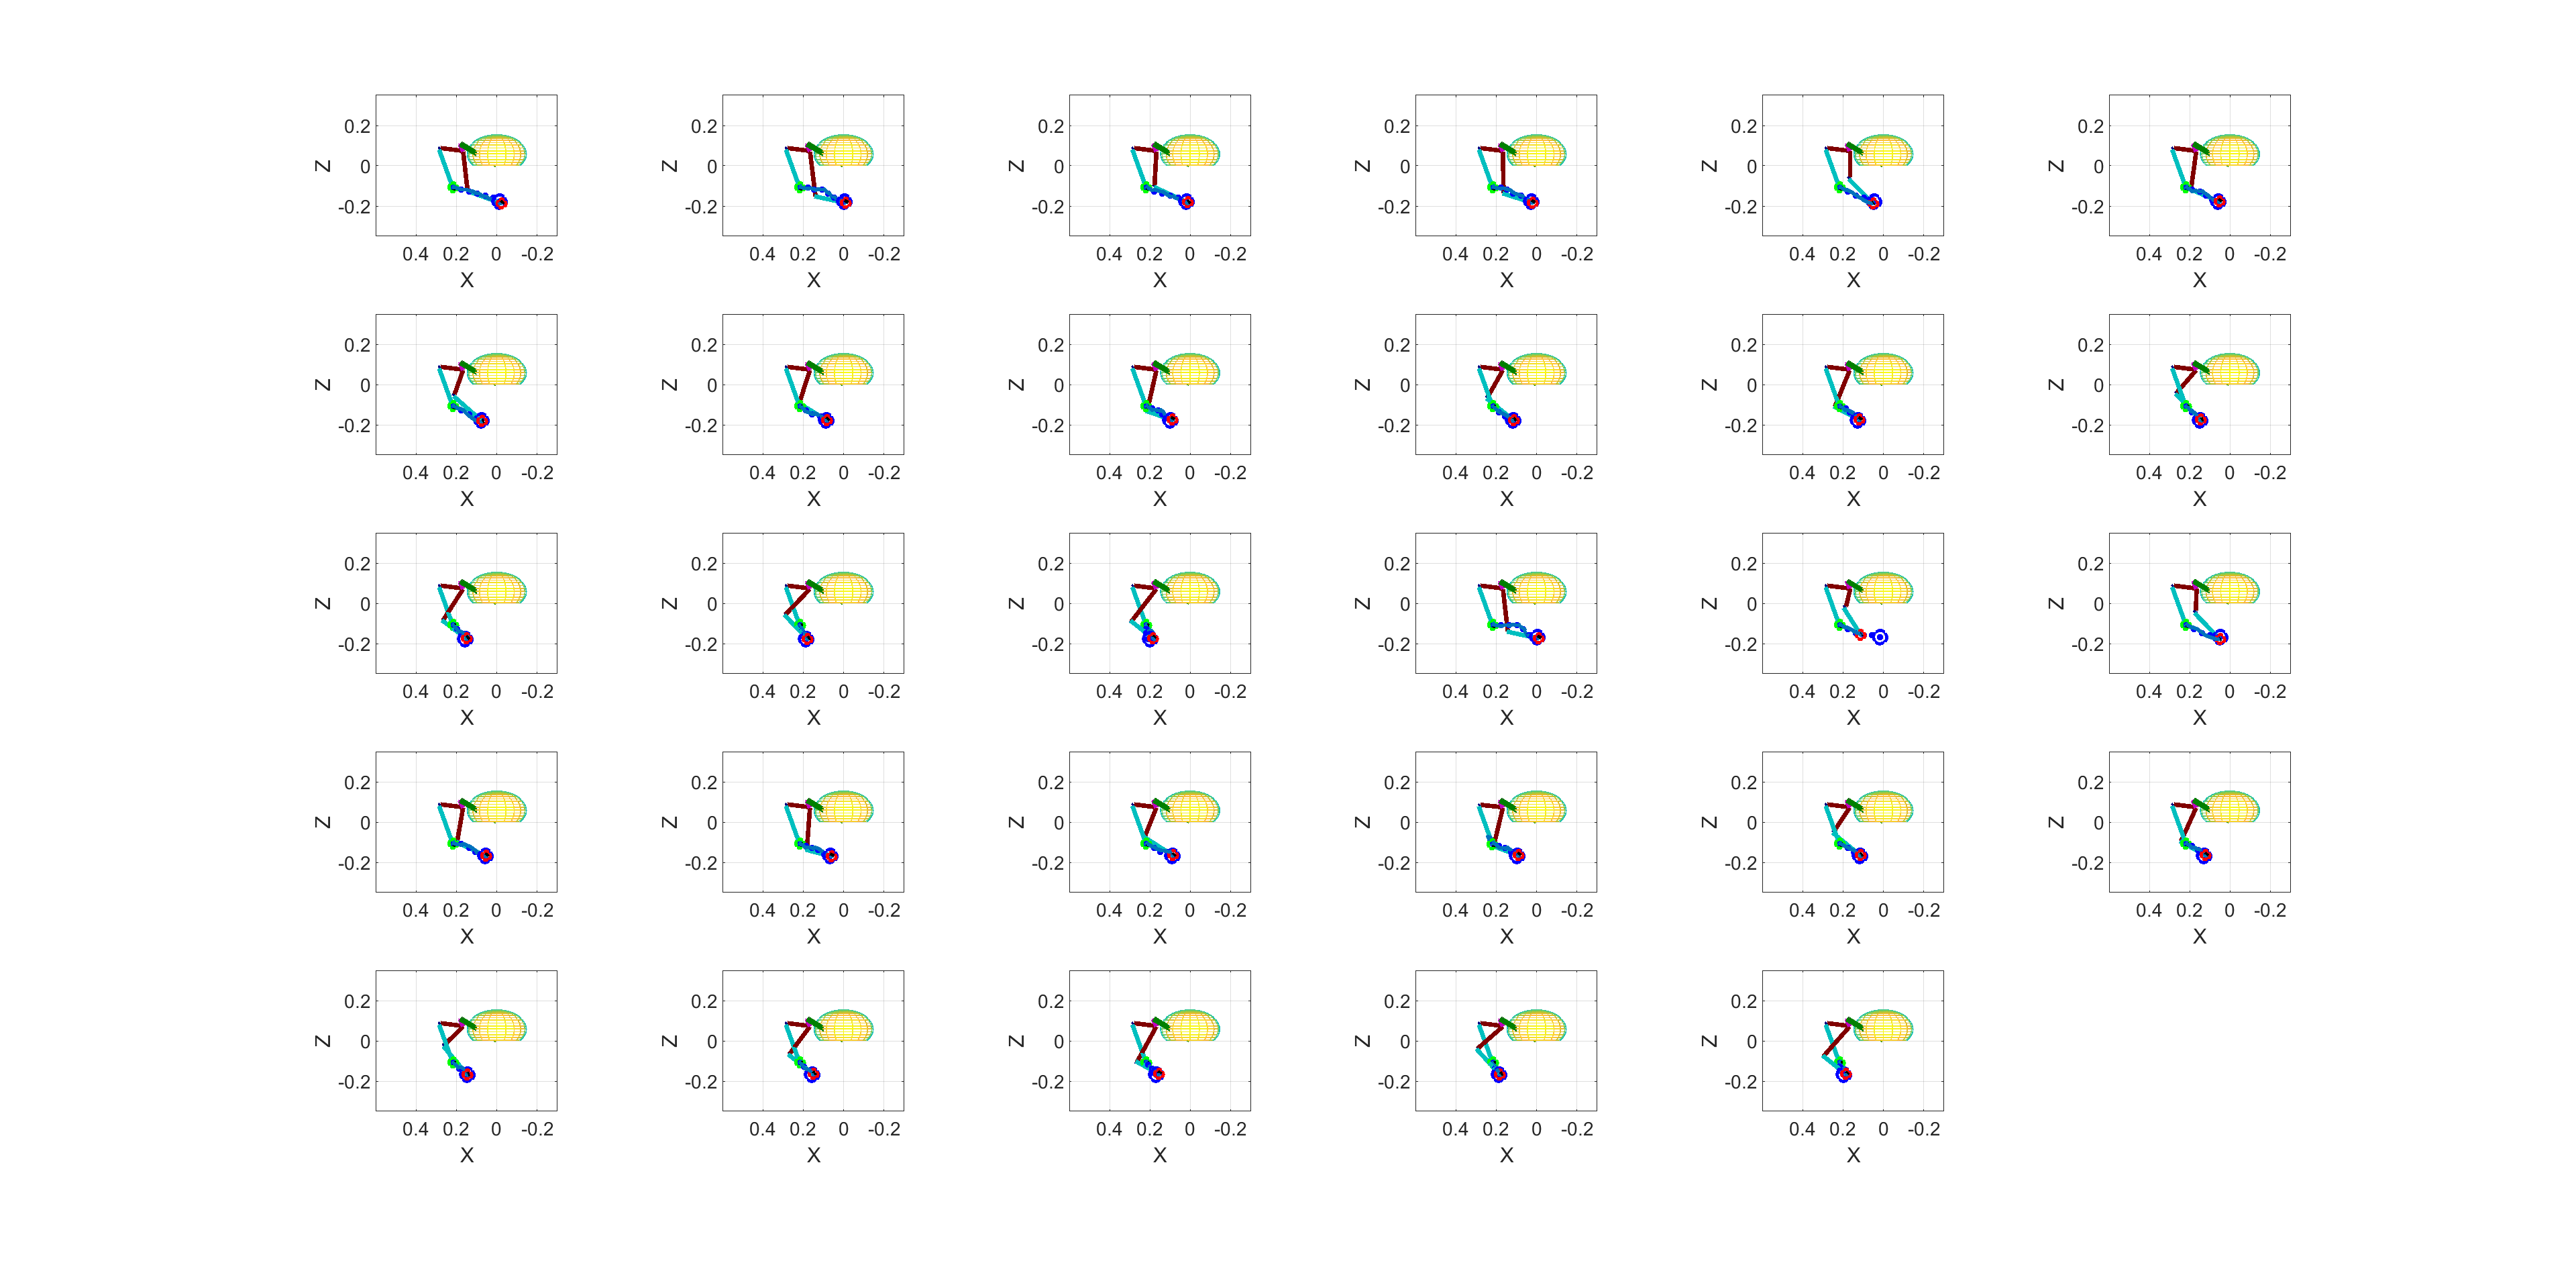
\includegraphics[width=1.7\textwidth]{Pictures/Results/Controller/QSC29positions.png}
    \caption{Desired Targets in Path-Following Quasi-Static Control} 
  \end{figure}
\end{landscape} % End landscape page

\subsection{EMG-Influenced Control}

\begin{figure}[h!]
\centering
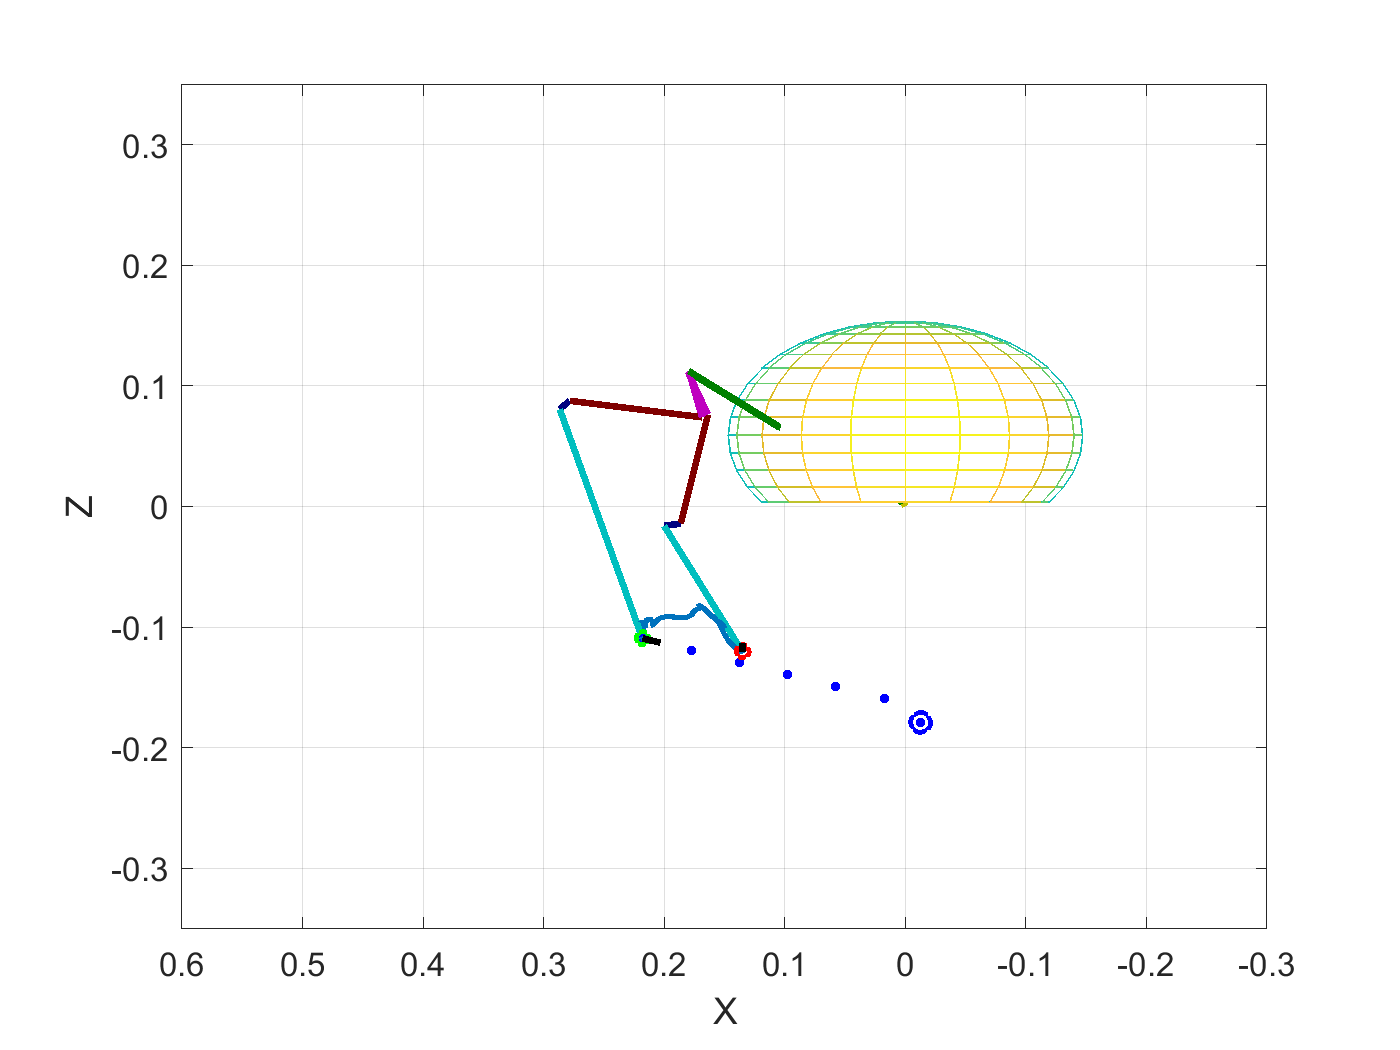
\includegraphics[width=0.75\textwidth]{Pictures/Results/Controller/StrokeWithouControl_WP.png} 
\caption{Stroke = 7 Without EMG-Influence Control Wrist Position} % Optional caption
\label{fig:WOEMGWP} % Optional label for referencing
\end{figure}

\begin{figure}[h!]
\centering
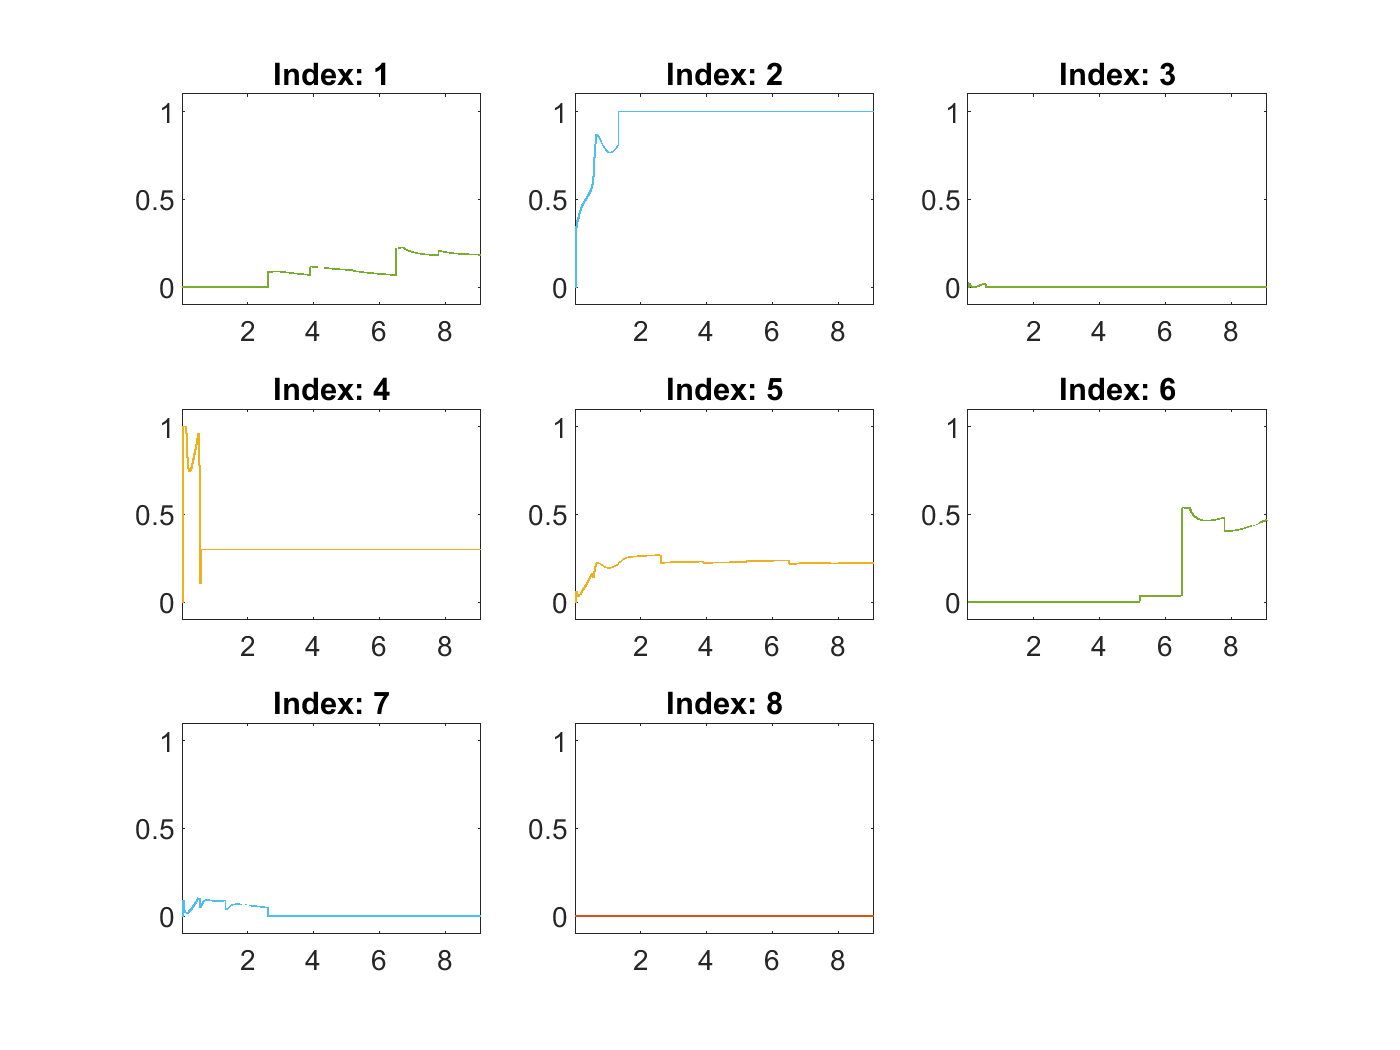
\includegraphics[width=1\textwidth]{Pictures/Results/Controller/StrokeWithouControl_NA.png} 
\caption{Stroke = 7 Without EMG-Influence Control Neural Activation} % Optional caption
\label{fig:WOEMGNA} % Optional label for referencing
\end{figure}


\newpage
\begin{landscape} % Start landscape page
  \begin{figure}[h!]
    \centering
    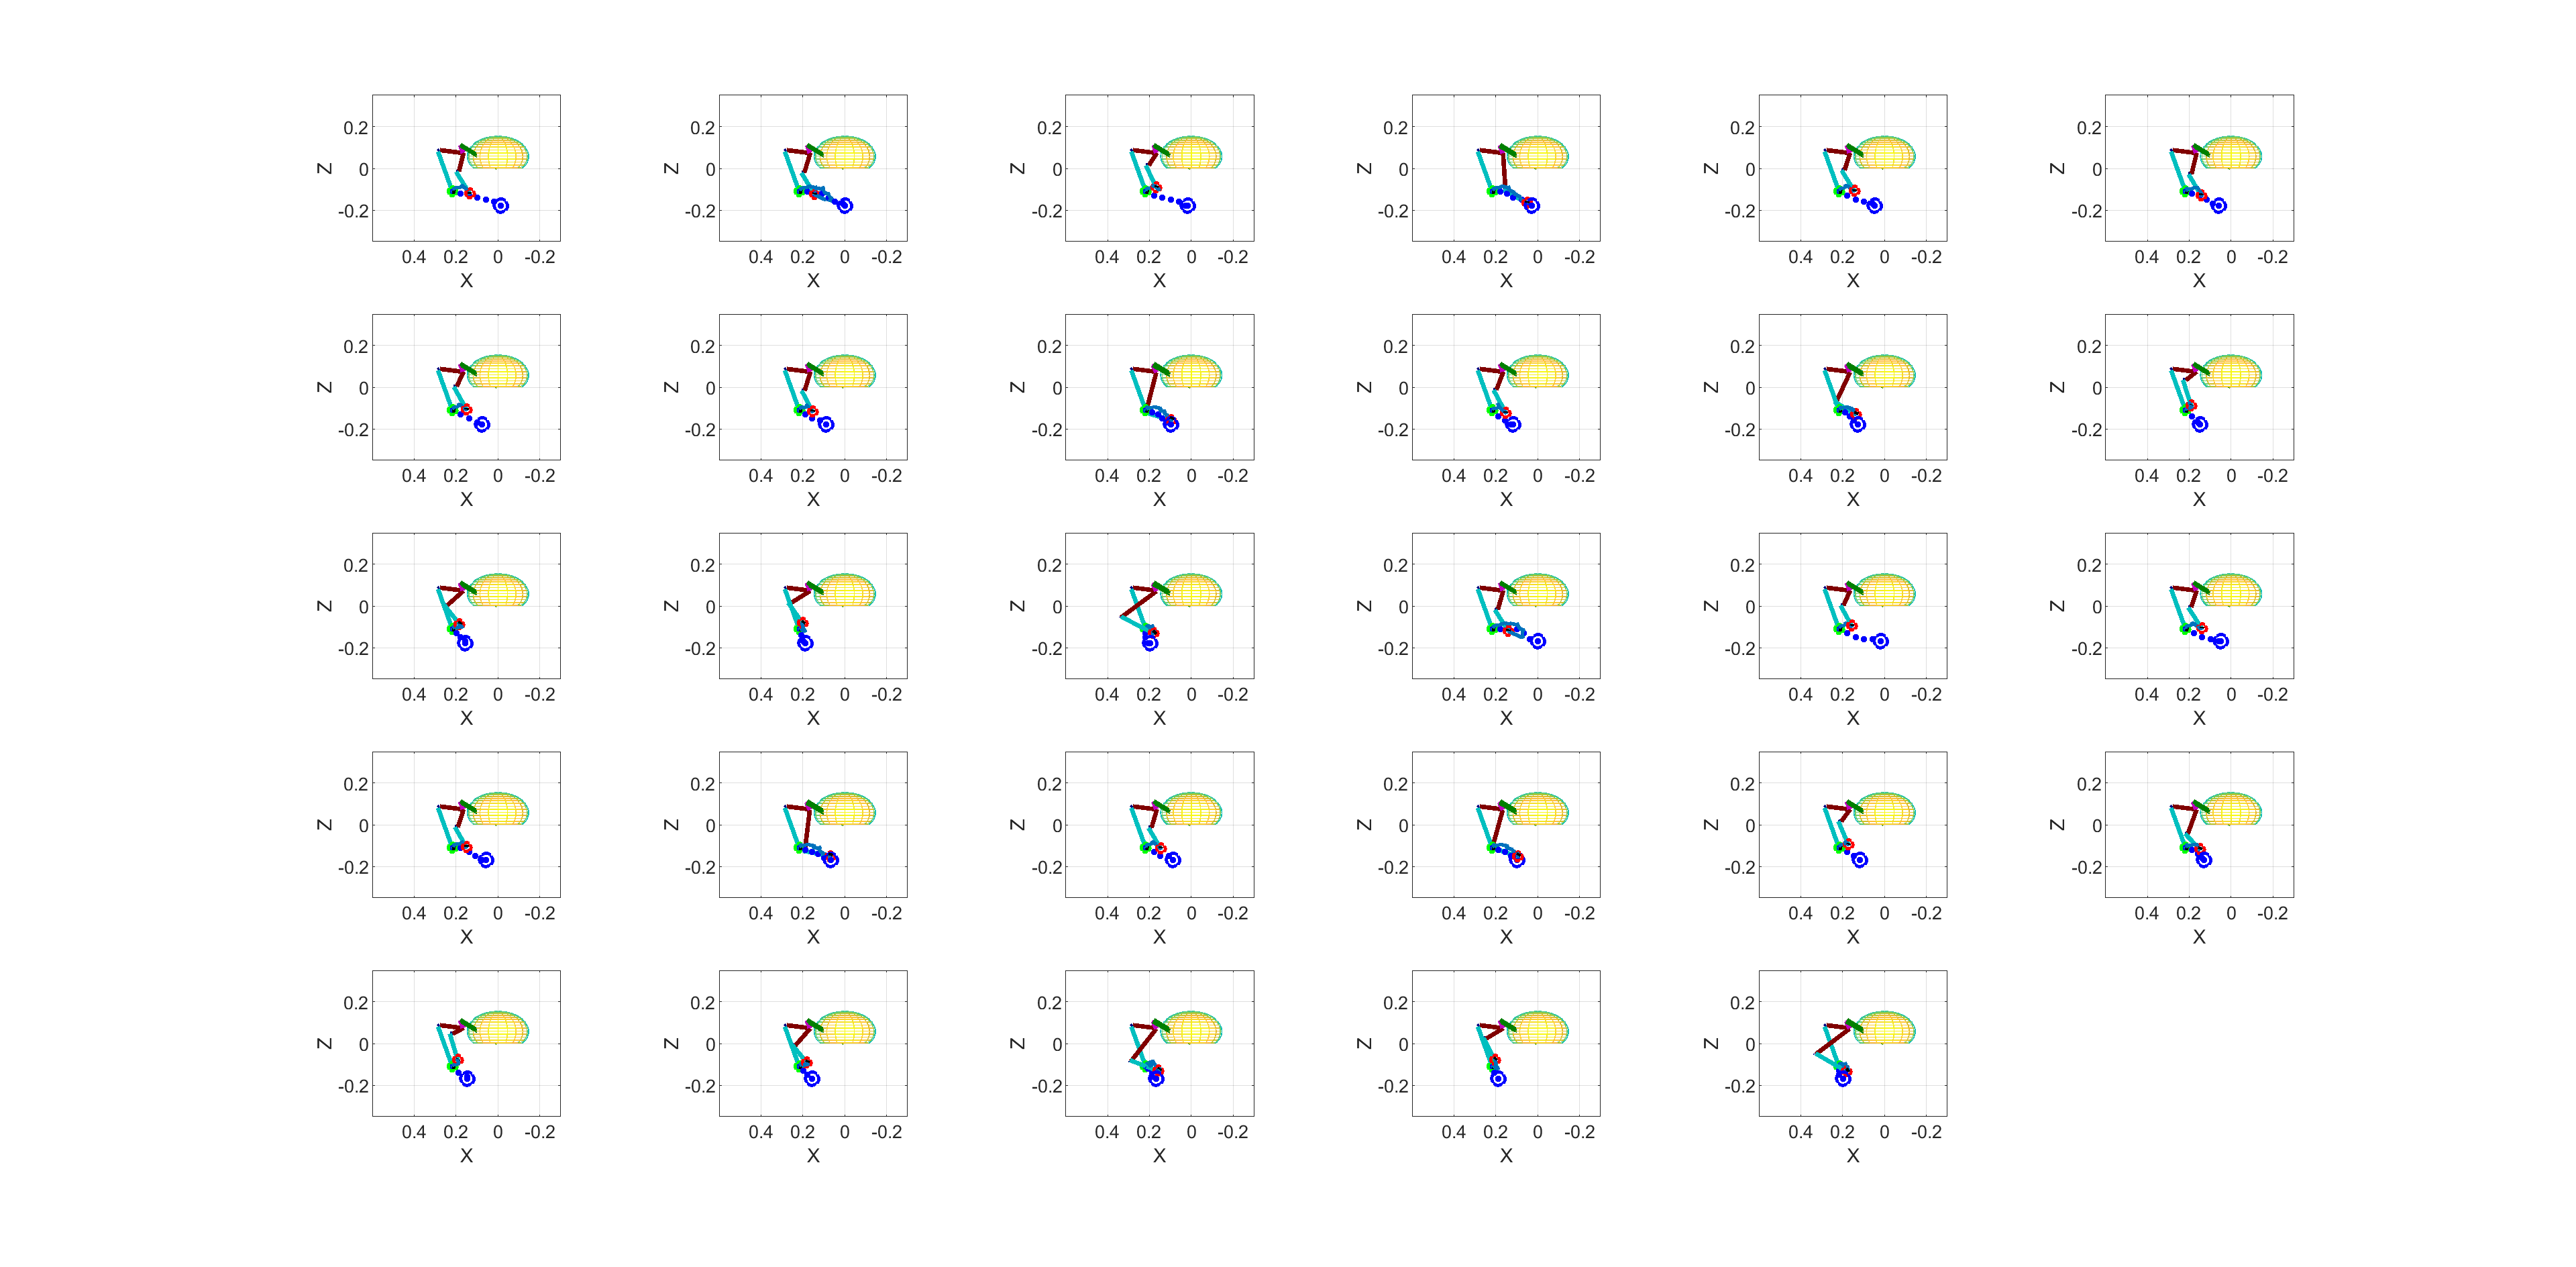
\includegraphics[width=1.9\textwidth]{Pictures/Results/Controller/WithStroke29positions.png} % Replace "filename.jpg" with the name of your image file
    \caption{Desired Targets With Stroke = 7 Without EMG-Influenced Control} % Optional caption
  \end{figure}
\end{landscape} % End landscape page


\begin{figure}[h!]
\centering
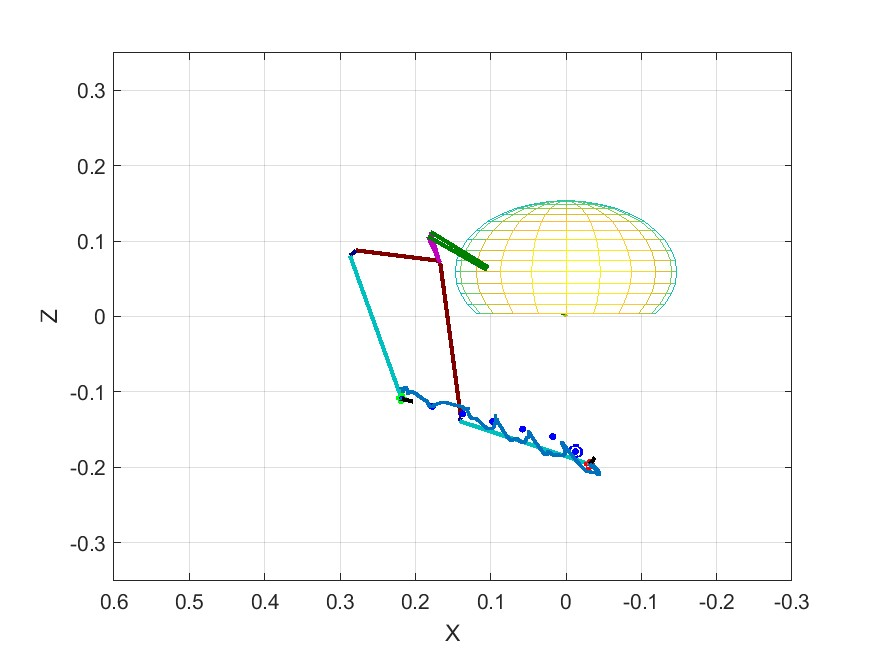
\includegraphics[width=0.75\textwidth]{Pictures/Results/Controller/G(2.99)_G(14.48)_Stroke_7_position_totry(5485)_wp.jpg} 
\caption{Stroke = 7 With EMG-Influence Control Wrist Position} % Optional caption
\label{fig:EMGWP} % Optional label for referencing
\end{figure}

\begin{figure}[h!]
\centering
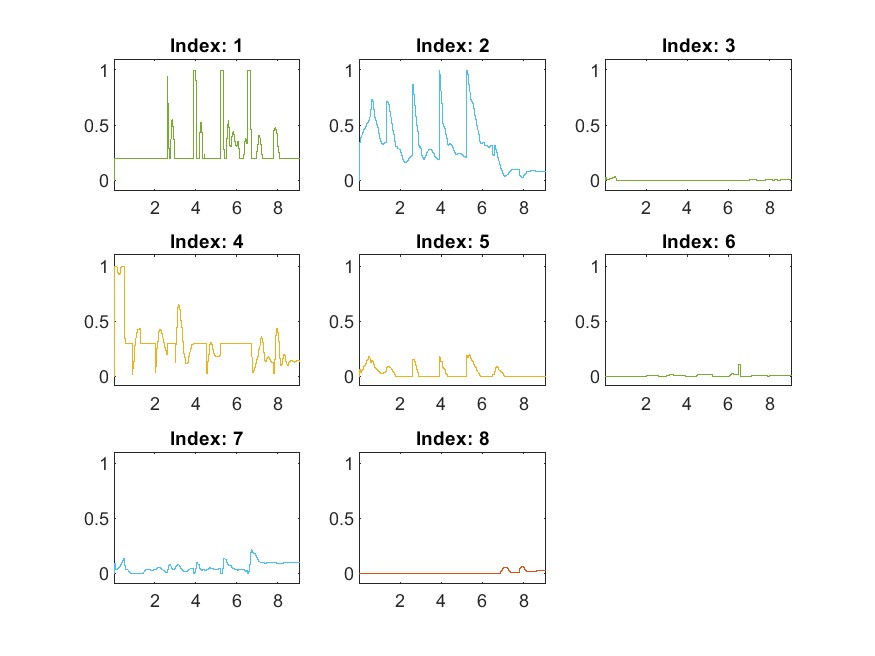
\includegraphics[width=1\textwidth]{Pictures/Results/Controller/G(2.99)_G(14.48)_Stroke_7_position_totry(5485).png_ne.jpg} 
\caption{Stroke = 7 With EMG-Influence Control Neural Activation} % Optional caption
\label{fig:EMGNA} % Optional label for referencing
\end{figure}

\begin{figure}[h!]
\centering
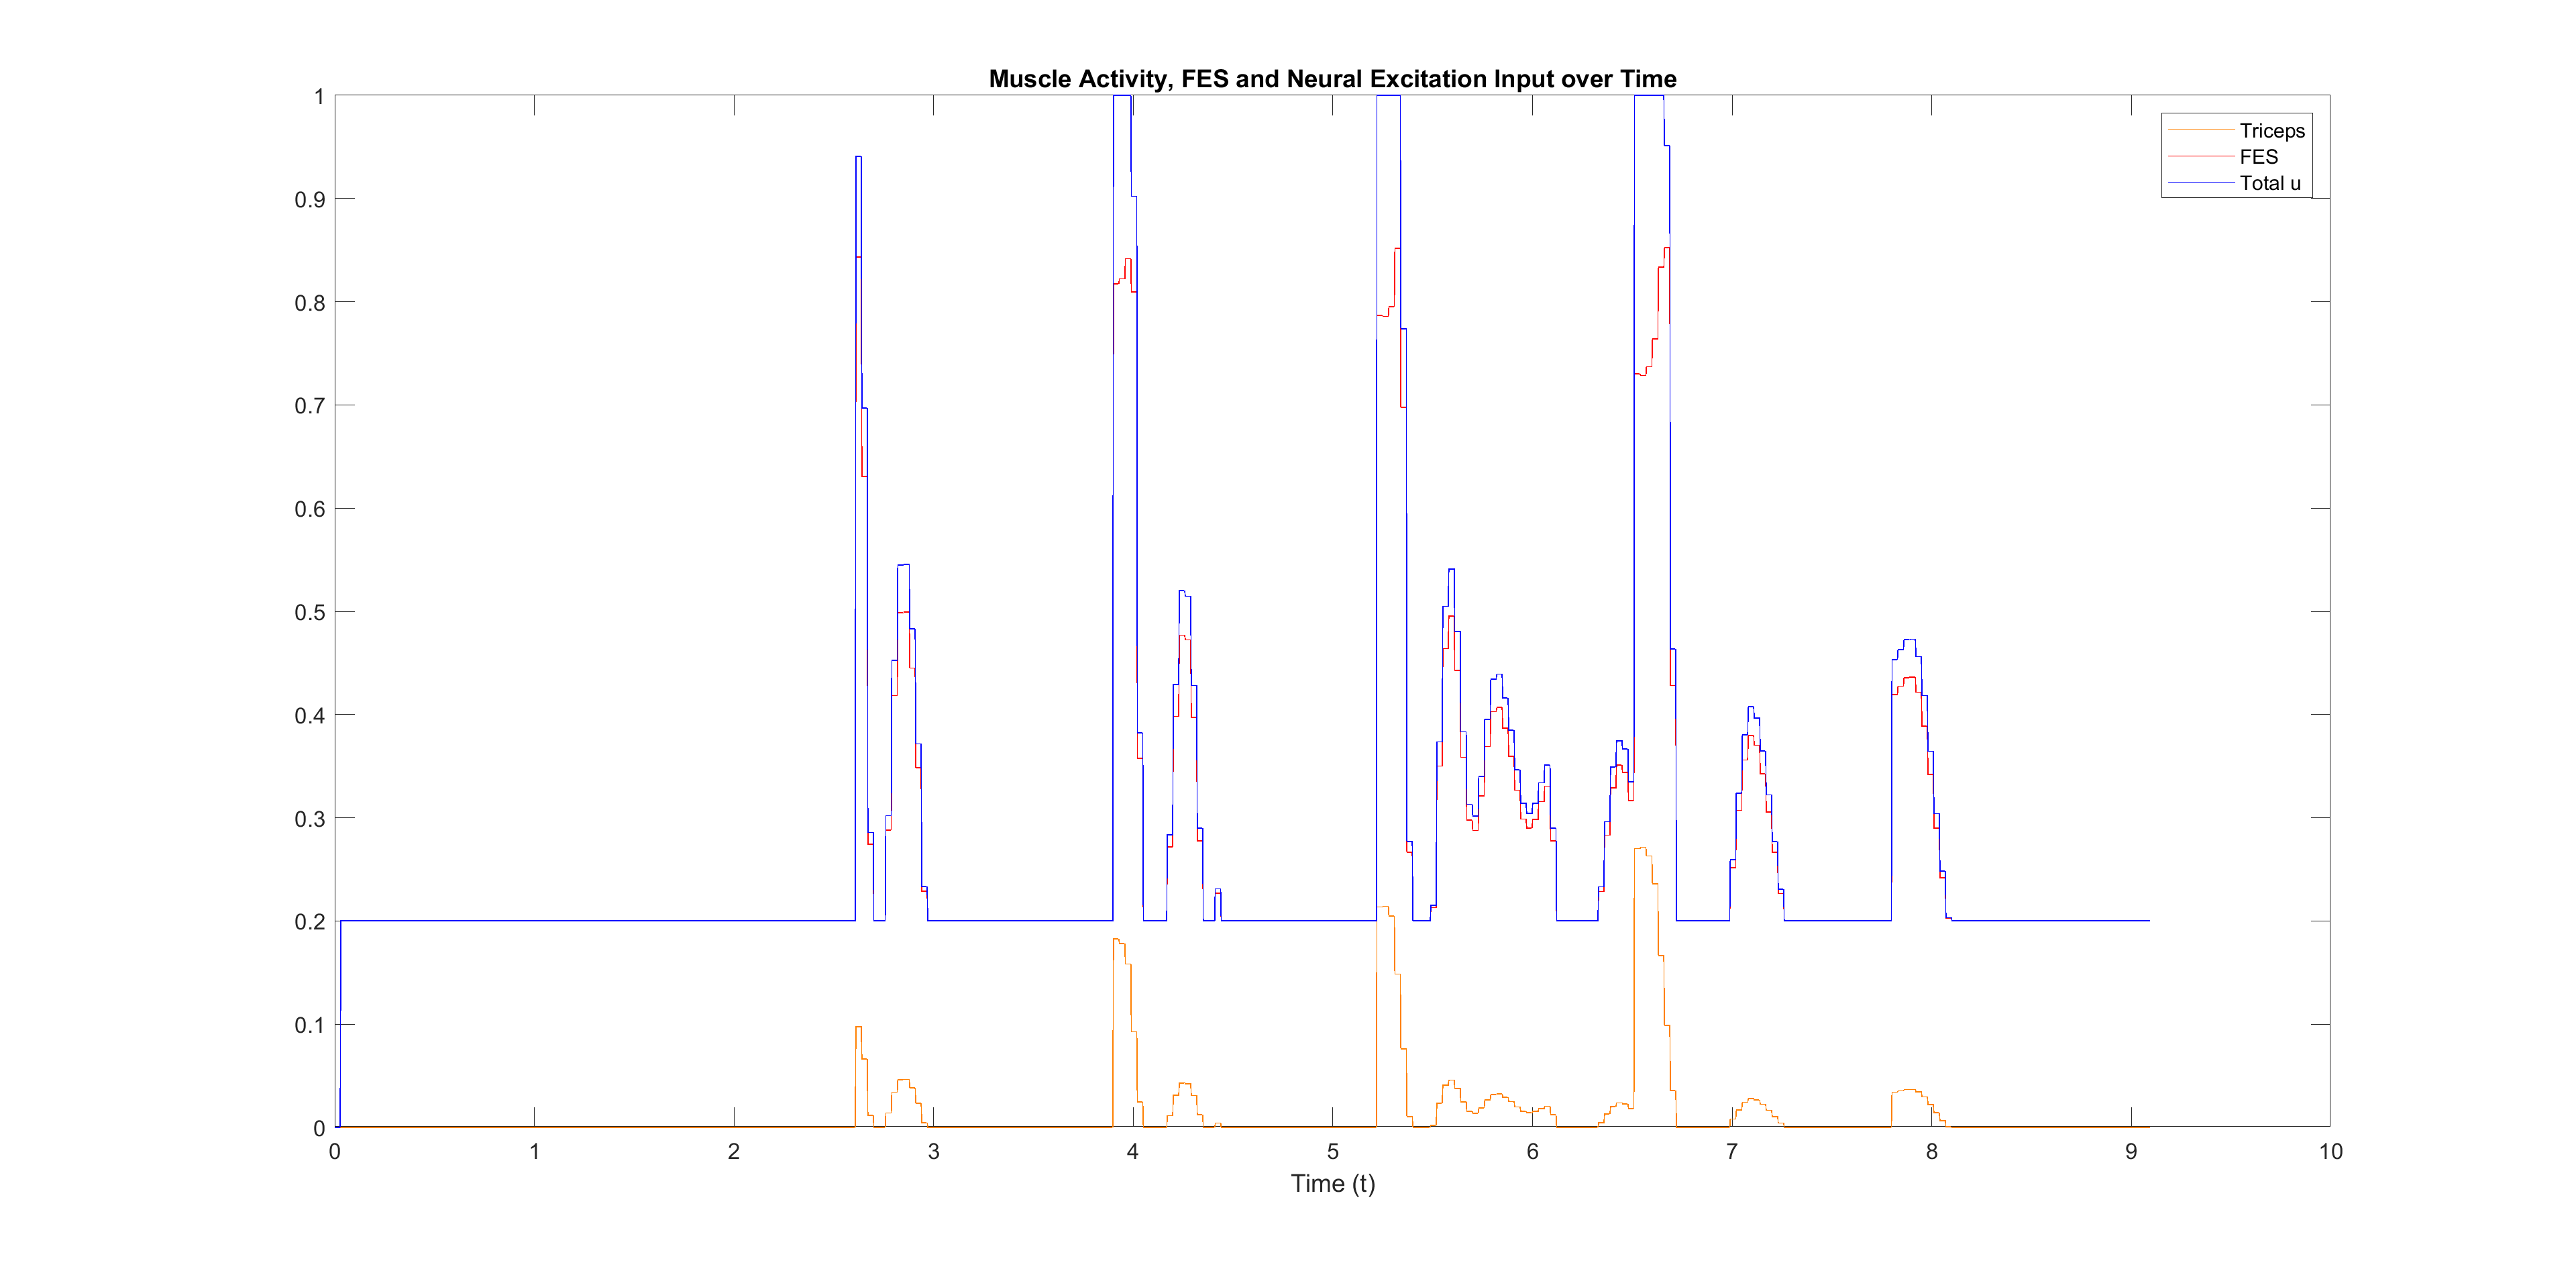
\includegraphics[width=\textwidth]{Pictures/Results/Controller/FESMuscleExcitations.png}
\caption{Triceps Activity, FES and Total Neural Excitation Over Time} 
\end{figure}

\newpage
\begin{landscape} % Start landscape page
  \begin{figure}[h!]
    \centering
    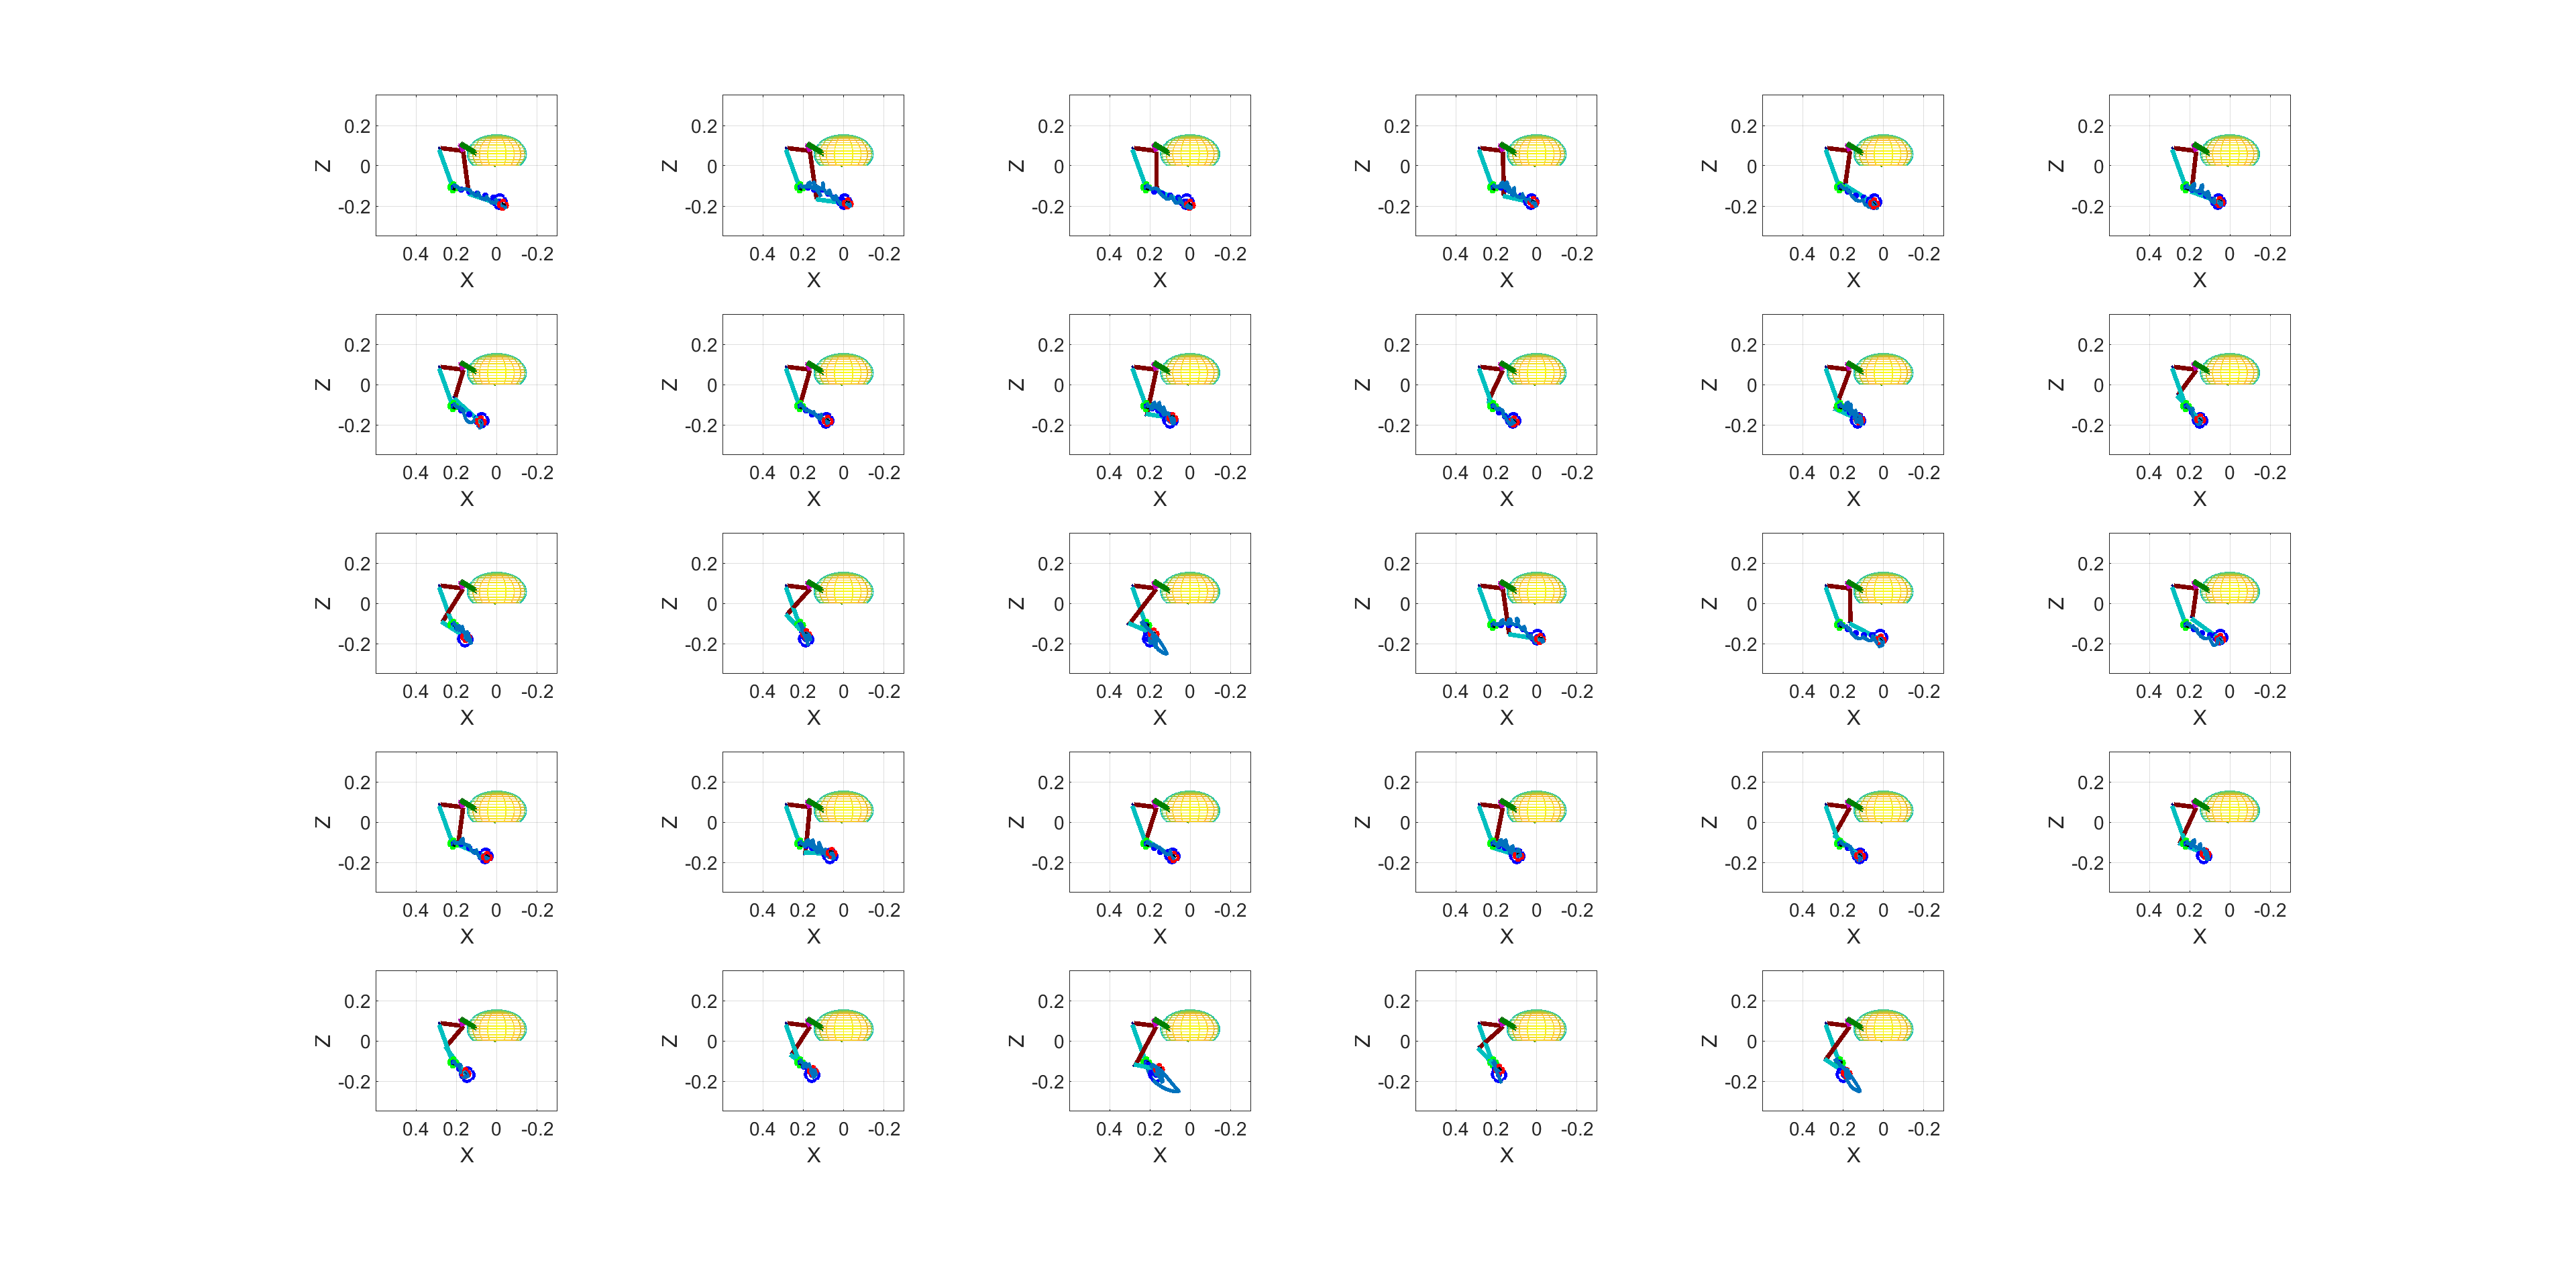
\includegraphics[width=1.9\textwidth]{Pictures/Results/Controller/Stroke29positions.png}
    \caption{Desired Targets With Stroke = 7 With EMG-Influenced Control} 
  \end{figure}
\end{landscape} % End landscape page